% Created by tikzDevice version 0.7.0 on 2014-06-29 16:56:15
% !TEX encoding = UTF-8 Unicode
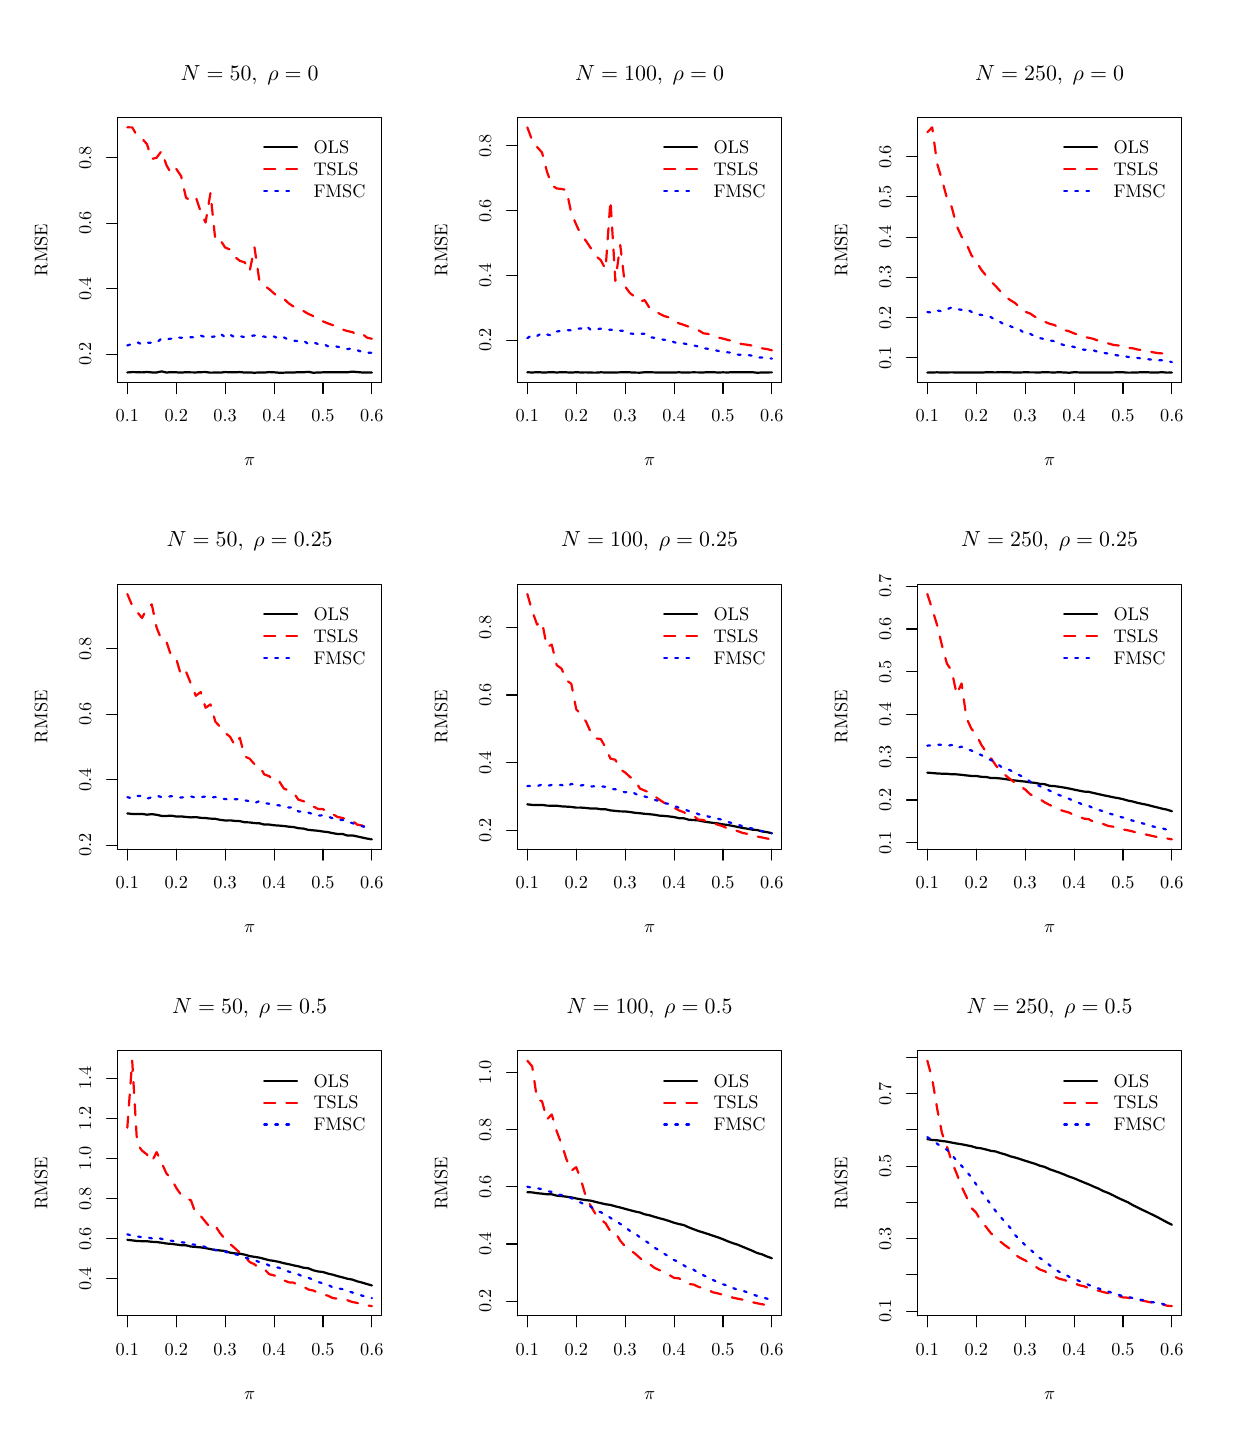
\begin{tikzpicture}[x=1pt,y=1pt]
\definecolor[named]{fillColor}{rgb}{1.00,1.00,1.00}
\path[use as bounding box,fill=fillColor,fill opacity=0.00] (0,0) rectangle (433.62,505.89);
\begin{scope}
\path[clip] ( 32.47,377.65) rectangle (127.91,473.42);
\definecolor[named]{drawColor}{rgb}{0.00,0.00,0.00}

\path[draw=drawColor,line width= 0.8pt,line join=round,line cap=round] ( 36.01,381.30) --
	( 37.77,381.43) --
	( 39.54,381.40) --
	( 41.31,381.32) --
	( 43.08,381.46) --
	( 44.84,381.32) --
	( 46.61,381.30) --
	( 48.38,381.68) --
	( 50.15,381.28) --
	( 51.91,381.41) --
	( 53.68,381.35) --
	( 55.45,381.24) --
	( 57.21,381.40) --
	( 58.98,381.33) --
	( 60.75,381.31) --
	( 62.52,381.40) --
	( 64.28,381.44) --
	( 66.05,381.23) --
	( 67.82,381.26) --
	( 69.59,381.24) --
	( 71.35,381.44) --
	( 73.12,381.36) --
	( 74.89,381.35) --
	( 76.66,381.44) --
	( 78.42,381.27) --
	( 80.19,381.30) --
	( 81.96,381.20) --
	( 83.72,381.30) --
	( 85.49,381.25) --
	( 87.26,381.43) --
	( 89.03,381.35) --
	( 90.79,381.21) --
	( 92.56,381.23) --
	( 94.33,381.28) --
	( 96.10,381.28) --
	( 97.86,381.40) --
	( 99.63,381.37) --
	(101.40,381.52) --
	(103.17,381.20) --
	(104.93,381.28) --
	(106.70,381.34) --
	(108.47,381.35) --
	(110.23,381.41) --
	(112.00,381.34) --
	(113.77,381.34) --
	(115.54,381.35) --
	(117.30,381.60) --
	(119.07,381.45) --
	(120.84,381.29) --
	(122.61,381.30) --
	(124.37,381.26);
\end{scope}
\begin{scope}
\path[clip] (  0.00,  0.00) rectangle (433.62,505.89);
\definecolor[named]{drawColor}{rgb}{0.00,0.00,0.00}

\path[draw=drawColor,line width= 0.4pt,line join=round,line cap=round] ( 36.01,377.65) -- (124.37,377.65);

\path[draw=drawColor,line width= 0.4pt,line join=round,line cap=round] ( 36.01,377.65) -- ( 36.01,373.69);

\path[draw=drawColor,line width= 0.4pt,line join=round,line cap=round] ( 53.68,377.65) -- ( 53.68,373.69);

\path[draw=drawColor,line width= 0.4pt,line join=round,line cap=round] ( 71.35,377.65) -- ( 71.35,373.69);

\path[draw=drawColor,line width= 0.4pt,line join=round,line cap=round] ( 89.03,377.65) -- ( 89.03,373.69);

\path[draw=drawColor,line width= 0.4pt,line join=round,line cap=round] (106.70,377.65) -- (106.70,373.69);

\path[draw=drawColor,line width= 0.4pt,line join=round,line cap=round] (124.37,377.65) -- (124.37,373.69);

\node[text=drawColor,anchor=base,inner sep=0pt, outer sep=0pt, scale=  0.66] at ( 36.01,363.40) {0.1};

\node[text=drawColor,anchor=base,inner sep=0pt, outer sep=0pt, scale=  0.66] at ( 53.68,363.40) {0.2};

\node[text=drawColor,anchor=base,inner sep=0pt, outer sep=0pt, scale=  0.66] at ( 71.35,363.40) {0.3};

\node[text=drawColor,anchor=base,inner sep=0pt, outer sep=0pt, scale=  0.66] at ( 89.03,363.40) {0.4};

\node[text=drawColor,anchor=base,inner sep=0pt, outer sep=0pt, scale=  0.66] at (106.70,363.40) {0.5};

\node[text=drawColor,anchor=base,inner sep=0pt, outer sep=0pt, scale=  0.66] at (124.37,363.40) {0.6};

\path[draw=drawColor,line width= 0.4pt,line join=round,line cap=round] ( 32.47,387.93) -- ( 32.47,458.95);

\path[draw=drawColor,line width= 0.4pt,line join=round,line cap=round] ( 32.47,387.93) -- ( 28.51,387.93);

\path[draw=drawColor,line width= 0.4pt,line join=round,line cap=round] ( 32.47,411.61) -- ( 28.51,411.61);

\path[draw=drawColor,line width= 0.4pt,line join=round,line cap=round] ( 32.47,435.28) -- ( 28.51,435.28);

\path[draw=drawColor,line width= 0.4pt,line join=round,line cap=round] ( 32.47,458.95) -- ( 28.51,458.95);

\node[text=drawColor,rotate= 90.00,anchor=base,inner sep=0pt, outer sep=0pt, scale=  0.66] at ( 22.97,387.93) {0.2};

\node[text=drawColor,rotate= 90.00,anchor=base,inner sep=0pt, outer sep=0pt, scale=  0.66] at ( 22.97,411.61) {0.4};

\node[text=drawColor,rotate= 90.00,anchor=base,inner sep=0pt, outer sep=0pt, scale=  0.66] at ( 22.97,435.28) {0.6};

\node[text=drawColor,rotate= 90.00,anchor=base,inner sep=0pt, outer sep=0pt, scale=  0.66] at ( 22.97,458.95) {0.8};

\path[draw=drawColor,line width= 0.4pt,line join=round,line cap=round] ( 32.47,377.65) --
	(127.91,377.65) --
	(127.91,473.42) --
	( 32.47,473.42) --
	( 32.47,377.65);
\end{scope}
\begin{scope}
\path[clip] (  0.00,337.26) rectangle (144.54,505.89);
\definecolor[named]{drawColor}{rgb}{0.00,0.00,0.00}

\node[text=drawColor,anchor=base,inner sep=0pt, outer sep=0pt, scale=  0.79] at ( 80.19,486.92) {\bfseries $N=50, \;\rho=0$};

\node[text=drawColor,anchor=base,inner sep=0pt, outer sep=0pt, scale=  0.66] at ( 80.19,347.56) {$\pi$};

\node[text=drawColor,rotate= 90.00,anchor=base,inner sep=0pt, outer sep=0pt, scale=  0.66] at (  7.13,425.53) {RMSE};
\end{scope}
\begin{scope}
\path[clip] ( 32.47,377.65) rectangle (127.91,473.42);
\definecolor[named]{drawColor}{rgb}{1.00,0.00,0.00}

\path[draw=drawColor,line width= 0.8pt,dash pattern=on 4pt off 4pt ,line join=round,line cap=round] ( 36.01,469.87) --
	( 37.77,469.85) --
	( 39.54,466.86) --
	( 41.31,465.84) --
	( 43.08,463.82) --
	( 44.84,458.41) --
	( 46.61,458.92) --
	( 48.38,461.32) --
	( 50.15,456.19) --
	( 51.91,453.08) --
	( 53.68,454.87) --
	( 55.45,452.24) --
	( 57.21,444.45) --
	( 58.98,443.41) --
	( 60.75,444.65) --
	( 62.52,439.39) --
	( 64.28,435.47) --
	( 66.05,446.15) --
	( 67.82,428.98) --
	( 69.59,429.16) --
	( 71.35,426.45) --
	( 73.12,425.71) --
	( 74.89,423.07) --
	( 76.66,421.62) --
	( 78.42,421.10) --
	( 80.19,417.78) --
	( 81.96,426.49) --
	( 83.72,414.46) --
	( 85.49,412.64) --
	( 87.26,411.44) --
	( 89.03,409.84) --
	( 90.79,408.38) --
	( 92.56,407.94) --
	( 94.33,406.26) --
	( 96.10,405.09) --
	( 97.86,404.67) --
	( 99.63,403.50) --
	(101.40,402.48) --
	(103.17,401.67) --
	(104.93,400.42) --
	(106.70,399.76) --
	(108.47,399.03) --
	(110.23,398.40) --
	(112.00,397.62) --
	(113.77,396.84) --
	(115.54,396.25) --
	(117.30,395.87) --
	(119.07,395.03) --
	(120.84,395.32) --
	(122.61,393.87) --
	(124.37,393.48);
\definecolor[named]{drawColor}{rgb}{0.00,0.00,1.00}

\path[draw=drawColor,line width= 0.8pt,dash pattern=on 1pt off 3pt ,line join=round,line cap=round] ( 36.01,391.05) --
	( 37.77,391.63) --
	( 39.54,392.26) --
	( 41.31,391.41) --
	( 43.08,392.08) --
	( 44.84,392.00) --
	( 46.61,392.05) --
	( 48.38,393.60) --
	( 50.15,393.29) --
	( 51.91,393.53) --
	( 53.68,394.01) --
	( 55.45,393.84) --
	( 57.21,394.09) --
	( 58.98,394.03) --
	( 60.75,393.97) --
	( 62.52,394.62) --
	( 64.28,394.04) --
	( 66.05,394.14) --
	( 67.82,394.31) --
	( 69.59,395.39) --
	( 71.35,393.99) --
	( 73.12,394.97) --
	( 74.89,393.96) --
	( 76.66,394.41) --
	( 78.42,394.07) --
	( 80.19,394.41) --
	( 81.96,394.68) --
	( 83.72,394.31) --
	( 85.49,394.26) --
	( 87.26,393.75) --
	( 89.03,394.28) --
	( 90.79,393.45) --
	( 92.56,394.00) --
	( 94.33,393.07) --
	( 96.10,392.77) --
	( 97.86,392.61) --
	( 99.63,392.80) --
	(101.40,391.58) --
	(103.17,392.17) --
	(104.93,391.57) --
	(106.70,391.68) --
	(108.47,390.78) --
	(110.23,390.88) --
	(112.00,390.59) --
	(113.77,390.26) --
	(115.54,389.75) --
	(117.30,389.99) --
	(119.07,389.35) --
	(120.84,388.68) --
	(122.61,388.39) --
	(124.37,388.44);
\definecolor[named]{drawColor}{rgb}{0.00,0.00,0.00}

\path[draw=drawColor,line width= 0.8pt,line join=round,line cap=round] ( 85.47,462.63) -- ( 97.35,462.63);
\definecolor[named]{drawColor}{rgb}{1.00,0.00,0.00}

\path[draw=drawColor,line width= 0.8pt,dash pattern=on 4pt off 4pt ,line join=round,line cap=round] ( 85.47,454.71) -- ( 97.35,454.71);
\definecolor[named]{drawColor}{rgb}{0.00,0.00,1.00}

\path[draw=drawColor,line width= 0.8pt,dash pattern=on 1pt off 3pt ,line join=round,line cap=round] ( 85.47,446.79) -- ( 97.35,446.79);
\definecolor[named]{drawColor}{rgb}{0.00,0.00,0.00}

\node[text=drawColor,anchor=base west,inner sep=0pt, outer sep=0pt, scale=  0.66] at (103.29,460.35) {OLS};

\node[text=drawColor,anchor=base west,inner sep=0pt, outer sep=0pt, scale=  0.66] at (103.29,452.43) {TSLS};

\node[text=drawColor,anchor=base west,inner sep=0pt, outer sep=0pt, scale=  0.66] at (103.29,444.51) {FMSC};
\end{scope}
\begin{scope}
\path[clip] ( 32.47,209.02) rectangle (127.91,304.79);
\definecolor[named]{drawColor}{rgb}{0.00,0.00,0.00}

\path[draw=drawColor,line width= 0.8pt,line join=round,line cap=round] ( 36.01,221.95) --
	( 37.77,221.77) --
	( 39.54,221.74) --
	( 41.31,221.79) --
	( 43.08,221.50) --
	( 44.84,221.70) --
	( 46.61,221.46) --
	( 48.38,221.06) --
	( 50.15,221.04) --
	( 51.91,221.16) --
	( 53.68,220.83) --
	( 55.45,220.88) --
	( 57.21,220.68) --
	( 58.98,220.52) --
	( 60.75,220.63) --
	( 62.52,220.36) --
	( 64.28,220.28) --
	( 66.05,220.08) --
	( 67.82,220.00) --
	( 69.59,219.62) --
	( 71.35,219.41) --
	( 73.12,219.45) --
	( 74.89,219.26) --
	( 76.66,219.17) --
	( 78.42,218.76) --
	( 80.19,218.71) --
	( 81.96,218.46) --
	( 83.72,218.40) --
	( 85.49,217.92) --
	( 87.26,217.94) --
	( 89.03,217.67) --
	( 90.79,217.56) --
	( 92.56,217.41) --
	( 94.33,217.17) --
	( 96.10,217.02) --
	( 97.86,216.61) --
	( 99.63,216.48) --
	(101.40,216.02) --
	(103.17,215.84) --
	(104.93,215.69) --
	(106.70,215.41) --
	(108.47,215.20) --
	(110.23,214.83) --
	(112.00,214.51) --
	(113.77,214.52) --
	(115.54,213.95) --
	(117.30,214.02) --
	(119.07,213.64) --
	(120.84,213.25) --
	(122.61,212.87) --
	(124.37,212.57);
\end{scope}
\begin{scope}
\path[clip] (  0.00,  0.00) rectangle (433.62,505.89);
\definecolor[named]{drawColor}{rgb}{0.00,0.00,0.00}

\path[draw=drawColor,line width= 0.4pt,line join=round,line cap=round] ( 36.01,209.02) -- (124.37,209.02);

\path[draw=drawColor,line width= 0.4pt,line join=round,line cap=round] ( 36.01,209.02) -- ( 36.01,205.06);

\path[draw=drawColor,line width= 0.4pt,line join=round,line cap=round] ( 53.68,209.02) -- ( 53.68,205.06);

\path[draw=drawColor,line width= 0.4pt,line join=round,line cap=round] ( 71.35,209.02) -- ( 71.35,205.06);

\path[draw=drawColor,line width= 0.4pt,line join=round,line cap=round] ( 89.03,209.02) -- ( 89.03,205.06);

\path[draw=drawColor,line width= 0.4pt,line join=round,line cap=round] (106.70,209.02) -- (106.70,205.06);

\path[draw=drawColor,line width= 0.4pt,line join=round,line cap=round] (124.37,209.02) -- (124.37,205.06);

\node[text=drawColor,anchor=base,inner sep=0pt, outer sep=0pt, scale=  0.66] at ( 36.01,194.77) {0.1};

\node[text=drawColor,anchor=base,inner sep=0pt, outer sep=0pt, scale=  0.66] at ( 53.68,194.77) {0.2};

\node[text=drawColor,anchor=base,inner sep=0pt, outer sep=0pt, scale=  0.66] at ( 71.35,194.77) {0.3};

\node[text=drawColor,anchor=base,inner sep=0pt, outer sep=0pt, scale=  0.66] at ( 89.03,194.77) {0.4};

\node[text=drawColor,anchor=base,inner sep=0pt, outer sep=0pt, scale=  0.66] at (106.70,194.77) {0.5};

\node[text=drawColor,anchor=base,inner sep=0pt, outer sep=0pt, scale=  0.66] at (124.37,194.77) {0.6};

\path[draw=drawColor,line width= 0.4pt,line join=round,line cap=round] ( 32.47,210.49) -- ( 32.47,281.43);

\path[draw=drawColor,line width= 0.4pt,line join=round,line cap=round] ( 32.47,210.49) -- ( 28.51,210.49);

\path[draw=drawColor,line width= 0.4pt,line join=round,line cap=round] ( 32.47,234.14) -- ( 28.51,234.14);

\path[draw=drawColor,line width= 0.4pt,line join=round,line cap=round] ( 32.47,257.79) -- ( 28.51,257.79);

\path[draw=drawColor,line width= 0.4pt,line join=round,line cap=round] ( 32.47,281.43) -- ( 28.51,281.43);

\node[text=drawColor,rotate= 90.00,anchor=base,inner sep=0pt, outer sep=0pt, scale=  0.66] at ( 22.97,210.49) {0.2};

\node[text=drawColor,rotate= 90.00,anchor=base,inner sep=0pt, outer sep=0pt, scale=  0.66] at ( 22.97,234.14) {0.4};

\node[text=drawColor,rotate= 90.00,anchor=base,inner sep=0pt, outer sep=0pt, scale=  0.66] at ( 22.97,257.79) {0.6};

\node[text=drawColor,rotate= 90.00,anchor=base,inner sep=0pt, outer sep=0pt, scale=  0.66] at ( 22.97,281.43) {0.8};

\path[draw=drawColor,line width= 0.4pt,line join=round,line cap=round] ( 32.47,209.02) --
	(127.91,209.02) --
	(127.91,304.79) --
	( 32.47,304.79) --
	( 32.47,209.02);
\end{scope}
\begin{scope}
\path[clip] (  0.00,168.63) rectangle (144.54,337.26);
\definecolor[named]{drawColor}{rgb}{0.00,0.00,0.00}

\node[text=drawColor,anchor=base,inner sep=0pt, outer sep=0pt, scale=  0.79] at ( 80.19,318.29) {\bfseries $N=50, \;\rho=0.25$};

\node[text=drawColor,anchor=base,inner sep=0pt, outer sep=0pt, scale=  0.66] at ( 80.19,178.93) {$\pi$};

\node[text=drawColor,rotate= 90.00,anchor=base,inner sep=0pt, outer sep=0pt, scale=  0.66] at (  7.13,256.90) {RMSE};
\end{scope}
\begin{scope}
\path[clip] ( 32.47,209.02) rectangle (127.91,304.79);
\definecolor[named]{drawColor}{rgb}{1.00,0.00,0.00}

\path[draw=drawColor,line width= 0.8pt,dash pattern=on 4pt off 4pt ,line join=round,line cap=round] ( 36.01,301.24) --
	( 37.77,297.05) --
	( 39.54,294.79) --
	( 41.31,292.57) --
	( 43.08,295.94) --
	( 44.84,297.50) --
	( 46.61,289.05) --
	( 48.38,284.67) --
	( 50.15,284.02) --
	( 51.91,278.71) --
	( 53.68,277.81) --
	( 55.45,271.81) --
	( 57.21,273.20) --
	( 58.98,268.86) --
	( 60.75,264.46) --
	( 62.52,265.84) --
	( 64.28,260.15) --
	( 66.05,261.34) --
	( 67.82,255.11) --
	( 69.59,253.20) --
	( 71.35,251.02) --
	( 73.12,249.68) --
	( 74.89,246.51) --
	( 76.66,249.28) --
	( 78.42,242.53) --
	( 80.19,241.76) --
	( 81.96,239.74) --
	( 83.72,239.08) --
	( 85.49,236.05) --
	( 87.26,235.43) --
	( 89.03,233.66) --
	( 90.79,233.72) --
	( 92.56,230.94) --
	( 94.33,230.26) --
	( 96.10,229.40) --
	( 97.86,226.88) --
	( 99.63,226.41) --
	(101.40,225.41) --
	(103.17,224.50) --
	(104.93,223.58) --
	(106.70,223.52) --
	(108.47,222.24) --
	(110.23,221.71) --
	(112.00,220.65) --
	(113.77,220.34) --
	(115.54,219.55) --
	(117.30,219.40) --
	(119.07,217.91) --
	(120.84,217.57) --
	(122.61,216.74) --
	(124.37,216.35);
\definecolor[named]{drawColor}{rgb}{0.00,0.00,1.00}

\path[draw=drawColor,line width= 0.8pt,dash pattern=on 1pt off 3pt ,line join=round,line cap=round] ( 36.01,227.85) --
	( 37.77,227.38) --
	( 39.54,228.29) --
	( 41.31,228.29) --
	( 43.08,227.26) --
	( 44.84,227.85) --
	( 46.61,228.39) --
	( 48.38,227.84) --
	( 50.15,227.92) --
	( 51.91,228.18) --
	( 53.68,227.86) --
	( 55.45,227.69) --
	( 57.21,227.93) --
	( 58.98,228.09) --
	( 60.75,227.65) --
	( 62.52,227.84) --
	( 64.28,228.06) --
	( 66.05,227.63) --
	( 67.82,227.89) --
	( 69.59,227.27) --
	( 71.35,227.17) --
	( 73.12,226.92) --
	( 74.89,227.09) --
	( 76.66,227.15) --
	( 78.42,226.69) --
	( 80.19,226.35) --
	( 81.96,225.65) --
	( 83.72,226.42) --
	( 85.49,225.70) --
	( 87.26,225.45) --
	( 89.03,224.96) --
	( 90.79,224.89) --
	( 92.56,224.38) --
	( 94.33,224.10) --
	( 96.10,224.19) --
	( 97.86,222.62) --
	( 99.63,222.69) --
	(101.40,222.25) --
	(103.17,221.72) --
	(104.93,221.12) --
	(106.70,221.32) --
	(108.47,220.85) --
	(110.23,220.17) --
	(112.00,219.63) --
	(113.77,219.60) --
	(115.54,218.90) --
	(117.30,218.49) --
	(119.07,217.61) --
	(120.84,217.37) --
	(122.61,216.72) --
	(124.37,216.41);
\definecolor[named]{drawColor}{rgb}{0.00,0.00,0.00}

\path[draw=drawColor,line width= 0.8pt,line join=round,line cap=round] ( 85.47,294.00) -- ( 97.35,294.00);
\definecolor[named]{drawColor}{rgb}{1.00,0.00,0.00}

\path[draw=drawColor,line width= 0.8pt,dash pattern=on 4pt off 4pt ,line join=round,line cap=round] ( 85.47,286.08) -- ( 97.35,286.08);
\definecolor[named]{drawColor}{rgb}{0.00,0.00,1.00}

\path[draw=drawColor,line width= 0.8pt,dash pattern=on 1pt off 3pt ,line join=round,line cap=round] ( 85.47,278.16) -- ( 97.35,278.16);
\definecolor[named]{drawColor}{rgb}{0.00,0.00,0.00}

\node[text=drawColor,anchor=base west,inner sep=0pt, outer sep=0pt, scale=  0.66] at (103.29,291.72) {OLS};

\node[text=drawColor,anchor=base west,inner sep=0pt, outer sep=0pt, scale=  0.66] at (103.29,283.80) {TSLS};

\node[text=drawColor,anchor=base west,inner sep=0pt, outer sep=0pt, scale=  0.66] at (103.29,275.88) {FMSC};
\end{scope}
\begin{scope}
\path[clip] ( 32.47, 40.39) rectangle (127.91,136.16);
\definecolor[named]{drawColor}{rgb}{0.00,0.00,0.00}

\path[draw=drawColor,line width= 0.8pt,line join=round,line cap=round] ( 36.01, 67.89) --
	( 37.77, 67.68) --
	( 39.54, 67.44) --
	( 41.31, 67.39) --
	( 43.08, 67.37) --
	( 44.84, 67.16) --
	( 46.61, 67.07) --
	( 48.38, 66.84) --
	( 50.15, 66.54) --
	( 51.91, 66.41) --
	( 53.68, 66.19) --
	( 55.45, 65.94) --
	( 57.21, 65.90) --
	( 58.98, 65.45) --
	( 60.75, 65.30) --
	( 62.52, 65.15) --
	( 64.28, 64.88) --
	( 66.05, 64.52) --
	( 67.82, 64.22) --
	( 69.59, 64.02) --
	( 71.35, 63.83) --
	( 73.12, 63.24) --
	( 74.89, 62.99) --
	( 76.66, 62.87) --
	( 78.42, 62.53) --
	( 80.19, 62.00) --
	( 81.96, 61.73) --
	( 83.72, 61.45) --
	( 85.49, 60.99) --
	( 87.26, 60.51) --
	( 89.03, 60.26) --
	( 90.79, 59.90) --
	( 92.56, 59.42) --
	( 94.33, 59.08) --
	( 96.10, 58.65) --
	( 97.86, 58.30) --
	( 99.63, 57.80) --
	(101.40, 57.60) --
	(103.17, 56.88) --
	(104.93, 56.44) --
	(106.70, 56.25) --
	(108.47, 55.68) --
	(110.23, 55.29) --
	(112.00, 54.75) --
	(113.77, 54.31) --
	(115.54, 53.82) --
	(117.30, 53.51) --
	(119.07, 52.88) --
	(120.84, 52.43) --
	(122.61, 51.90) --
	(124.37, 51.39);
\end{scope}
\begin{scope}
\path[clip] (  0.00,  0.00) rectangle (433.62,505.89);
\definecolor[named]{drawColor}{rgb}{0.00,0.00,0.00}

\path[draw=drawColor,line width= 0.4pt,line join=round,line cap=round] ( 36.01, 40.39) -- (124.37, 40.39);

\path[draw=drawColor,line width= 0.4pt,line join=round,line cap=round] ( 36.01, 40.39) -- ( 36.01, 36.43);

\path[draw=drawColor,line width= 0.4pt,line join=round,line cap=round] ( 53.68, 40.39) -- ( 53.68, 36.43);

\path[draw=drawColor,line width= 0.4pt,line join=round,line cap=round] ( 71.35, 40.39) -- ( 71.35, 36.43);

\path[draw=drawColor,line width= 0.4pt,line join=round,line cap=round] ( 89.03, 40.39) -- ( 89.03, 36.43);

\path[draw=drawColor,line width= 0.4pt,line join=round,line cap=round] (106.70, 40.39) -- (106.70, 36.43);

\path[draw=drawColor,line width= 0.4pt,line join=round,line cap=round] (124.37, 40.39) -- (124.37, 36.43);

\node[text=drawColor,anchor=base,inner sep=0pt, outer sep=0pt, scale=  0.66] at ( 36.01, 26.14) {0.1};

\node[text=drawColor,anchor=base,inner sep=0pt, outer sep=0pt, scale=  0.66] at ( 53.68, 26.14) {0.2};

\node[text=drawColor,anchor=base,inner sep=0pt, outer sep=0pt, scale=  0.66] at ( 71.35, 26.14) {0.3};

\node[text=drawColor,anchor=base,inner sep=0pt, outer sep=0pt, scale=  0.66] at ( 89.03, 26.14) {0.4};

\node[text=drawColor,anchor=base,inner sep=0pt, outer sep=0pt, scale=  0.66] at (106.70, 26.14) {0.5};

\node[text=drawColor,anchor=base,inner sep=0pt, outer sep=0pt, scale=  0.66] at (124.37, 26.14) {0.6};

\path[draw=drawColor,line width= 0.4pt,line join=round,line cap=round] ( 32.47, 53.79) -- ( 32.47,126.27);

\path[draw=drawColor,line width= 0.4pt,line join=round,line cap=round] ( 32.47, 53.79) -- ( 28.51, 53.79);

\path[draw=drawColor,line width= 0.4pt,line join=round,line cap=round] ( 32.47, 68.28) -- ( 28.51, 68.28);

\path[draw=drawColor,line width= 0.4pt,line join=round,line cap=round] ( 32.47, 82.78) -- ( 28.51, 82.78);

\path[draw=drawColor,line width= 0.4pt,line join=round,line cap=round] ( 32.47, 97.28) -- ( 28.51, 97.28);

\path[draw=drawColor,line width= 0.4pt,line join=round,line cap=round] ( 32.47,111.78) -- ( 28.51,111.78);

\path[draw=drawColor,line width= 0.4pt,line join=round,line cap=round] ( 32.47,126.27) -- ( 28.51,126.27);

\node[text=drawColor,rotate= 90.00,anchor=base,inner sep=0pt, outer sep=0pt, scale=  0.66] at ( 22.97, 53.79) {0.4};

\node[text=drawColor,rotate= 90.00,anchor=base,inner sep=0pt, outer sep=0pt, scale=  0.66] at ( 22.97, 68.28) {0.6};

\node[text=drawColor,rotate= 90.00,anchor=base,inner sep=0pt, outer sep=0pt, scale=  0.66] at ( 22.97, 82.78) {0.8};

\node[text=drawColor,rotate= 90.00,anchor=base,inner sep=0pt, outer sep=0pt, scale=  0.66] at ( 22.97, 97.28) {1.0};

\node[text=drawColor,rotate= 90.00,anchor=base,inner sep=0pt, outer sep=0pt, scale=  0.66] at ( 22.97,111.78) {1.2};

\node[text=drawColor,rotate= 90.00,anchor=base,inner sep=0pt, outer sep=0pt, scale=  0.66] at ( 22.97,126.27) {1.4};

\path[draw=drawColor,line width= 0.4pt,line join=round,line cap=round] ( 32.47, 40.39) --
	(127.91, 40.39) --
	(127.91,136.16) --
	( 32.47,136.16) --
	( 32.47, 40.39);
\end{scope}
\begin{scope}
\path[clip] (  0.00,  0.00) rectangle (144.54,168.63);
\definecolor[named]{drawColor}{rgb}{0.00,0.00,0.00}

\node[text=drawColor,anchor=base,inner sep=0pt, outer sep=0pt, scale=  0.79] at ( 80.19,149.66) {\bfseries $N=50, \;\rho=0.5$};

\node[text=drawColor,anchor=base,inner sep=0pt, outer sep=0pt, scale=  0.66] at ( 80.19, 10.30) {$\pi$};

\node[text=drawColor,rotate= 90.00,anchor=base,inner sep=0pt, outer sep=0pt, scale=  0.66] at (  7.13, 88.27) {RMSE};
\end{scope}
\begin{scope}
\path[clip] ( 32.47, 40.39) rectangle (127.91,136.16);
\definecolor[named]{drawColor}{rgb}{1.00,0.00,0.00}

\path[draw=drawColor,line width= 0.8pt,dash pattern=on 4pt off 4pt ,line join=round,line cap=round] ( 36.01,108.41) --
	( 37.77,132.61) --
	( 39.54,102.63) --
	( 41.31,100.10) --
	( 43.08, 98.74) --
	( 44.84, 96.14) --
	( 46.61, 99.57) --
	( 48.38, 95.74) --
	( 50.15, 91.85) --
	( 51.91, 89.94) --
	( 53.68, 86.67) --
	( 55.45, 84.10) --
	( 57.21, 82.77) --
	( 58.98, 82.18) --
	( 60.75, 77.27) --
	( 62.52, 76.48) --
	( 64.28, 74.35) --
	( 66.05, 72.20) --
	( 67.82, 72.86) --
	( 69.59, 70.23) --
	( 71.35, 68.07) --
	( 73.12, 66.41) --
	( 74.89, 64.84) --
	( 76.66, 63.21) --
	( 78.42, 61.84) --
	( 80.19, 59.86) --
	( 81.96, 59.03) --
	( 83.72, 57.63) --
	( 85.49, 57.34) --
	( 87.26, 55.48) --
	( 89.03, 55.01) --
	( 90.79, 54.54) --
	( 92.56, 53.27) --
	( 94.33, 52.52) --
	( 96.10, 52.40) --
	( 97.86, 51.39) --
	( 99.63, 50.97) --
	(101.40, 49.92) --
	(103.17, 49.58) --
	(104.93, 48.75) --
	(106.70, 48.06) --
	(108.47, 47.71) --
	(110.23, 46.84) --
	(112.00, 46.60) --
	(113.77, 46.49) --
	(115.54, 46.05) --
	(117.30, 45.41) --
	(119.07, 45.08) --
	(120.84, 44.43) --
	(122.61, 44.20) --
	(124.37, 43.94);
\definecolor[named]{drawColor}{rgb}{0.00,0.00,1.00}

\path[draw=drawColor,line width= 0.8pt,dash pattern=on 1pt off 3pt ,line join=round,line cap=round] ( 36.01, 69.87) --
	( 37.77, 69.38) --
	( 39.54, 69.10) --
	( 41.31, 68.86) --
	( 43.08, 68.77) --
	( 44.84, 68.41) --
	( 46.61, 68.68) --
	( 48.38, 68.21) --
	( 50.15, 67.87) --
	( 51.91, 67.56) --
	( 53.68, 67.18) --
	( 55.45, 67.01) --
	( 57.21, 66.80) --
	( 58.98, 66.31) --
	( 60.75, 66.07) --
	( 62.52, 65.94) --
	( 64.28, 65.23) --
	( 66.05, 64.77) --
	( 67.82, 64.15) --
	( 69.59, 64.05) --
	( 71.35, 63.63) --
	( 73.12, 62.90) --
	( 74.89, 62.68) --
	( 76.66, 62.29) --
	( 78.42, 61.52) --
	( 80.19, 60.95) --
	( 81.96, 60.51) --
	( 83.72, 59.85) --
	( 85.49, 59.53) --
	( 87.26, 58.59) --
	( 89.03, 57.98) --
	( 90.79, 57.81) --
	( 92.56, 56.91) --
	( 94.33, 56.39) --
	( 96.10, 55.80) --
	( 97.86, 55.37) --
	( 99.63, 54.51) --
	(101.40, 54.20) --
	(103.17, 53.43) --
	(104.93, 52.63) --
	(106.70, 52.16) --
	(108.47, 51.68) --
	(110.23, 50.69) --
	(112.00, 50.35) --
	(113.77, 50.05) --
	(115.54, 49.44) --
	(117.30, 48.84) --
	(119.07, 48.42) --
	(120.84, 47.69) --
	(122.61, 47.35) --
	(124.37, 46.80);
\definecolor[named]{drawColor}{rgb}{0.00,0.00,0.00}

\path[draw=drawColor,line width= 0.8pt,line join=round,line cap=round] ( 85.47,125.37) -- ( 97.35,125.37);
\definecolor[named]{drawColor}{rgb}{1.00,0.00,0.00}

\path[draw=drawColor,line width= 0.8pt,dash pattern=on 4pt off 4pt ,line join=round,line cap=round] ( 85.47,117.45) -- ( 97.35,117.45);
\definecolor[named]{drawColor}{rgb}{0.00,0.00,1.00}

\path[draw=drawColor,line width= 0.8pt,dash pattern=on 1pt off 3pt ,line join=round,line cap=round] ( 85.47,109.53) -- ( 97.35,109.53);
\definecolor[named]{drawColor}{rgb}{0.00,0.00,0.00}

\node[text=drawColor,anchor=base west,inner sep=0pt, outer sep=0pt, scale=  0.66] at (103.29,123.09) {OLS};

\node[text=drawColor,anchor=base west,inner sep=0pt, outer sep=0pt, scale=  0.66] at (103.29,115.17) {TSLS};

\node[text=drawColor,anchor=base west,inner sep=0pt, outer sep=0pt, scale=  0.66] at (103.29,107.25) {FMSC};
\end{scope}
\begin{scope}
\path[clip] (177.01,377.65) rectangle (272.45,473.42);
\definecolor[named]{drawColor}{rgb}{0.00,0.00,0.00}

\path[draw=drawColor,line width= 0.8pt,line join=round,line cap=round] (180.55,381.37) --
	(182.31,381.28) --
	(184.08,381.40) --
	(185.85,381.31) --
	(187.62,381.32) --
	(189.38,381.41) --
	(191.15,381.29) --
	(192.92,381.39) --
	(194.69,381.34) --
	(196.45,381.27) --
	(198.22,381.37) --
	(199.99,381.30) --
	(201.75,381.33) --
	(203.52,381.25) --
	(205.29,381.23) --
	(207.06,381.35) --
	(208.82,381.29) --
	(210.59,381.30) --
	(212.36,381.29) --
	(214.13,381.34) --
	(215.89,381.38) --
	(217.66,381.34) --
	(219.43,381.25) --
	(221.20,381.22) --
	(222.96,381.37) --
	(224.73,381.37) --
	(226.50,381.32) --
	(228.26,381.26) --
	(230.03,381.32) --
	(231.80,381.30) --
	(233.57,381.28) --
	(235.33,381.35) --
	(237.10,381.28) --
	(238.87,381.31) --
	(240.64,381.34) --
	(242.40,381.32) --
	(244.17,381.30) --
	(245.94,381.40) --
	(247.71,381.37) --
	(249.47,381.29) --
	(251.24,381.34) --
	(253.01,381.30) --
	(254.77,381.40) --
	(256.54,381.37) --
	(258.31,381.34) --
	(260.08,381.37) --
	(261.84,381.38) --
	(263.61,381.20) --
	(265.38,381.28) --
	(267.15,381.31) --
	(268.91,381.33);
\end{scope}
\begin{scope}
\path[clip] (  0.00,  0.00) rectangle (433.62,505.89);
\definecolor[named]{drawColor}{rgb}{0.00,0.00,0.00}

\path[draw=drawColor,line width= 0.4pt,line join=round,line cap=round] (180.55,377.65) -- (268.91,377.65);

\path[draw=drawColor,line width= 0.4pt,line join=round,line cap=round] (180.55,377.65) -- (180.55,373.69);

\path[draw=drawColor,line width= 0.4pt,line join=round,line cap=round] (198.22,377.65) -- (198.22,373.69);

\path[draw=drawColor,line width= 0.4pt,line join=round,line cap=round] (215.89,377.65) -- (215.89,373.69);

\path[draw=drawColor,line width= 0.4pt,line join=round,line cap=round] (233.57,377.65) -- (233.57,373.69);

\path[draw=drawColor,line width= 0.4pt,line join=round,line cap=round] (251.24,377.65) -- (251.24,373.69);

\path[draw=drawColor,line width= 0.4pt,line join=round,line cap=round] (268.91,377.65) -- (268.91,373.69);

\node[text=drawColor,anchor=base,inner sep=0pt, outer sep=0pt, scale=  0.66] at (180.55,363.40) {0.1};

\node[text=drawColor,anchor=base,inner sep=0pt, outer sep=0pt, scale=  0.66] at (198.22,363.40) {0.2};

\node[text=drawColor,anchor=base,inner sep=0pt, outer sep=0pt, scale=  0.66] at (215.89,363.40) {0.3};

\node[text=drawColor,anchor=base,inner sep=0pt, outer sep=0pt, scale=  0.66] at (233.57,363.40) {0.4};

\node[text=drawColor,anchor=base,inner sep=0pt, outer sep=0pt, scale=  0.66] at (251.24,363.40) {0.5};

\node[text=drawColor,anchor=base,inner sep=0pt, outer sep=0pt, scale=  0.66] at (268.91,363.40) {0.6};

\path[draw=drawColor,line width= 0.4pt,line join=round,line cap=round] (177.01,392.92) -- (177.01,463.21);

\path[draw=drawColor,line width= 0.4pt,line join=round,line cap=round] (177.01,392.92) -- (173.05,392.92);

\path[draw=drawColor,line width= 0.4pt,line join=round,line cap=round] (177.01,416.35) -- (173.05,416.35);

\path[draw=drawColor,line width= 0.4pt,line join=round,line cap=round] (177.01,439.78) -- (173.05,439.78);

\path[draw=drawColor,line width= 0.4pt,line join=round,line cap=round] (177.01,463.21) -- (173.05,463.21);

\node[text=drawColor,rotate= 90.00,anchor=base,inner sep=0pt, outer sep=0pt, scale=  0.66] at (167.51,392.92) {0.2};

\node[text=drawColor,rotate= 90.00,anchor=base,inner sep=0pt, outer sep=0pt, scale=  0.66] at (167.51,416.35) {0.4};

\node[text=drawColor,rotate= 90.00,anchor=base,inner sep=0pt, outer sep=0pt, scale=  0.66] at (167.51,439.78) {0.6};

\node[text=drawColor,rotate= 90.00,anchor=base,inner sep=0pt, outer sep=0pt, scale=  0.66] at (167.51,463.21) {0.8};

\path[draw=drawColor,line width= 0.4pt,line join=round,line cap=round] (177.01,377.65) --
	(272.45,377.65) --
	(272.45,473.42) --
	(177.01,473.42) --
	(177.01,377.65);
\end{scope}
\begin{scope}
\path[clip] (144.54,337.26) rectangle (289.08,505.89);
\definecolor[named]{drawColor}{rgb}{0.00,0.00,0.00}

\node[text=drawColor,anchor=base,inner sep=0pt, outer sep=0pt, scale=  0.79] at (224.73,486.92) {\bfseries $N=100, \;\rho=0$};

\node[text=drawColor,anchor=base,inner sep=0pt, outer sep=0pt, scale=  0.66] at (224.73,347.56) {$\pi$};

\node[text=drawColor,rotate= 90.00,anchor=base,inner sep=0pt, outer sep=0pt, scale=  0.66] at (151.67,425.53) {RMSE};
\end{scope}
\begin{scope}
\path[clip] (177.01,377.65) rectangle (272.45,473.42);
\definecolor[named]{drawColor}{rgb}{1.00,0.00,0.00}

\path[draw=drawColor,line width= 0.8pt,dash pattern=on 4pt off 4pt ,line join=round,line cap=round] (180.55,469.87) --
	(182.31,465.13) --
	(184.08,462.77) --
	(185.85,460.77) --
	(187.62,453.95) --
	(189.38,448.94) --
	(191.15,447.79) --
	(192.92,447.61) --
	(194.69,447.20) --
	(196.45,438.85) --
	(198.22,434.72) --
	(199.99,430.88) --
	(201.75,428.83) --
	(203.52,426.14) --
	(205.29,423.38) --
	(207.06,421.91) --
	(208.82,418.64) --
	(210.59,443.54) --
	(212.36,414.36) --
	(214.13,427.33) --
	(215.89,412.34) --
	(217.66,409.94) --
	(219.43,408.64) --
	(221.20,406.96) --
	(222.96,407.41) --
	(224.73,404.59) --
	(226.50,403.94) --
	(228.26,402.53) --
	(230.03,401.67) --
	(231.80,401.17) --
	(233.57,400.00) --
	(235.33,399.05) --
	(237.10,398.48) --
	(238.87,397.83) --
	(240.64,396.97) --
	(242.40,396.52) --
	(244.17,395.45) --
	(245.94,395.21) --
	(247.71,394.62) --
	(249.47,393.91) --
	(251.24,393.54) --
	(253.01,393.04) --
	(254.77,392.64) --
	(256.54,391.90) --
	(258.31,391.53) --
	(260.08,391.30) --
	(261.84,390.99) --
	(263.61,390.16) --
	(265.38,390.01) --
	(267.15,389.75) --
	(268.91,389.30);
\definecolor[named]{drawColor}{rgb}{0.00,0.00,1.00}

\path[draw=drawColor,line width= 0.8pt,dash pattern=on 1pt off 3pt ,line join=round,line cap=round] (180.55,393.70) --
	(182.31,394.87) --
	(184.08,394.48) --
	(185.85,395.56) --
	(187.62,395.02) --
	(189.38,394.67) --
	(191.15,396.10) --
	(192.92,396.34) --
	(194.69,396.64) --
	(196.45,396.49) --
	(198.22,397.04) --
	(199.99,397.20) --
	(201.75,398.17) --
	(203.52,396.62) --
	(205.29,396.84) --
	(207.06,397.14) --
	(208.82,396.59) --
	(210.59,396.78) --
	(212.36,396.43) --
	(214.13,396.41) --
	(215.89,396.28) --
	(217.66,395.40) --
	(219.43,395.17) --
	(221.20,395.20) --
	(222.96,395.32) --
	(224.73,394.04) --
	(226.50,393.82) --
	(228.26,393.43) --
	(230.03,393.08) --
	(231.80,393.09) --
	(233.57,392.22) --
	(235.33,391.73) --
	(237.10,391.75) --
	(238.87,391.42) --
	(240.64,391.09) --
	(242.40,390.63) --
	(244.17,389.98) --
	(245.94,389.87) --
	(247.71,389.50) --
	(249.47,389.09) --
	(251.24,388.81) --
	(253.01,388.56) --
	(254.77,388.42) --
	(256.54,387.76) --
	(258.31,387.61) --
	(260.08,387.61) --
	(261.84,387.35) --
	(263.61,386.69) --
	(265.38,386.68) --
	(267.15,386.49) --
	(268.91,386.30);
\definecolor[named]{drawColor}{rgb}{0.00,0.00,0.00}

\path[draw=drawColor,line width= 0.8pt,line join=round,line cap=round] (230.01,462.63) -- (241.89,462.63);
\definecolor[named]{drawColor}{rgb}{1.00,0.00,0.00}

\path[draw=drawColor,line width= 0.8pt,dash pattern=on 4pt off 4pt ,line join=round,line cap=round] (230.01,454.71) -- (241.89,454.71);
\definecolor[named]{drawColor}{rgb}{0.00,0.00,1.00}

\path[draw=drawColor,line width= 0.8pt,dash pattern=on 1pt off 3pt ,line join=round,line cap=round] (230.01,446.79) -- (241.89,446.79);
\definecolor[named]{drawColor}{rgb}{0.00,0.00,0.00}

\node[text=drawColor,anchor=base west,inner sep=0pt, outer sep=0pt, scale=  0.66] at (247.83,460.35) {OLS};

\node[text=drawColor,anchor=base west,inner sep=0pt, outer sep=0pt, scale=  0.66] at (247.83,452.43) {TSLS};

\node[text=drawColor,anchor=base west,inner sep=0pt, outer sep=0pt, scale=  0.66] at (247.83,444.51) {FMSC};
\end{scope}
\begin{scope}
\path[clip] (177.01,209.02) rectangle (272.45,304.79);
\definecolor[named]{drawColor}{rgb}{0.00,0.00,0.00}

\path[draw=drawColor,line width= 0.8pt,line join=round,line cap=round] (180.55,225.25) --
	(182.31,225.03) --
	(184.08,224.99) --
	(185.85,225.03) --
	(187.62,224.78) --
	(189.38,224.74) --
	(191.15,224.74) --
	(192.92,224.51) --
	(194.69,224.41) --
	(196.45,224.30) --
	(198.22,224.05) --
	(199.99,224.06) --
	(201.75,223.94) --
	(203.52,223.71) --
	(205.29,223.76) --
	(207.06,223.49) --
	(208.82,223.45) --
	(210.59,223.05) --
	(212.36,222.87) --
	(214.13,222.70) --
	(215.89,222.67) --
	(217.66,222.46) --
	(219.43,222.19) --
	(221.20,222.03) --
	(222.96,221.81) --
	(224.73,221.68) --
	(226.50,221.48) --
	(228.26,221.16) --
	(230.03,221.05) --
	(231.80,220.87) --
	(233.57,220.64) --
	(235.33,220.25) --
	(237.10,220.19) --
	(238.87,219.68) --
	(240.64,219.56) --
	(242.40,219.42) --
	(244.17,219.04) --
	(245.94,218.77) --
	(247.71,218.54) --
	(249.47,218.33) --
	(251.24,217.99) --
	(253.01,217.78) --
	(254.77,217.43) --
	(256.54,217.08) --
	(258.31,216.71) --
	(260.08,216.43) --
	(261.84,216.09) --
	(263.61,215.96) --
	(265.38,215.45) --
	(267.15,215.19) --
	(268.91,214.82);
\end{scope}
\begin{scope}
\path[clip] (  0.00,  0.00) rectangle (433.62,505.89);
\definecolor[named]{drawColor}{rgb}{0.00,0.00,0.00}

\path[draw=drawColor,line width= 0.4pt,line join=round,line cap=round] (180.55,209.02) -- (268.91,209.02);

\path[draw=drawColor,line width= 0.4pt,line join=round,line cap=round] (180.55,209.02) -- (180.55,205.06);

\path[draw=drawColor,line width= 0.4pt,line join=round,line cap=round] (198.22,209.02) -- (198.22,205.06);

\path[draw=drawColor,line width= 0.4pt,line join=round,line cap=round] (215.89,209.02) -- (215.89,205.06);

\path[draw=drawColor,line width= 0.4pt,line join=round,line cap=round] (233.57,209.02) -- (233.57,205.06);

\path[draw=drawColor,line width= 0.4pt,line join=round,line cap=round] (251.24,209.02) -- (251.24,205.06);

\path[draw=drawColor,line width= 0.4pt,line join=round,line cap=round] (268.91,209.02) -- (268.91,205.06);

\node[text=drawColor,anchor=base,inner sep=0pt, outer sep=0pt, scale=  0.66] at (180.55,194.77) {0.1};

\node[text=drawColor,anchor=base,inner sep=0pt, outer sep=0pt, scale=  0.66] at (198.22,194.77) {0.2};

\node[text=drawColor,anchor=base,inner sep=0pt, outer sep=0pt, scale=  0.66] at (215.89,194.77) {0.3};

\node[text=drawColor,anchor=base,inner sep=0pt, outer sep=0pt, scale=  0.66] at (233.57,194.77) {0.4};

\node[text=drawColor,anchor=base,inner sep=0pt, outer sep=0pt, scale=  0.66] at (251.24,194.77) {0.5};

\node[text=drawColor,anchor=base,inner sep=0pt, outer sep=0pt, scale=  0.66] at (268.91,194.77) {0.6};

\path[draw=drawColor,line width= 0.4pt,line join=round,line cap=round] (177.01,215.83) -- (177.01,289.18);

\path[draw=drawColor,line width= 0.4pt,line join=round,line cap=round] (177.01,215.83) -- (173.05,215.83);

\path[draw=drawColor,line width= 0.4pt,line join=round,line cap=round] (177.01,240.28) -- (173.05,240.28);

\path[draw=drawColor,line width= 0.4pt,line join=round,line cap=round] (177.01,264.73) -- (173.05,264.73);

\path[draw=drawColor,line width= 0.4pt,line join=round,line cap=round] (177.01,289.18) -- (173.05,289.18);

\node[text=drawColor,rotate= 90.00,anchor=base,inner sep=0pt, outer sep=0pt, scale=  0.66] at (167.51,215.83) {0.2};

\node[text=drawColor,rotate= 90.00,anchor=base,inner sep=0pt, outer sep=0pt, scale=  0.66] at (167.51,240.28) {0.4};

\node[text=drawColor,rotate= 90.00,anchor=base,inner sep=0pt, outer sep=0pt, scale=  0.66] at (167.51,264.73) {0.6};

\node[text=drawColor,rotate= 90.00,anchor=base,inner sep=0pt, outer sep=0pt, scale=  0.66] at (167.51,289.18) {0.8};

\path[draw=drawColor,line width= 0.4pt,line join=round,line cap=round] (177.01,209.02) --
	(272.45,209.02) --
	(272.45,304.79) --
	(177.01,304.79) --
	(177.01,209.02);
\end{scope}
\begin{scope}
\path[clip] (144.54,168.63) rectangle (289.08,337.26);
\definecolor[named]{drawColor}{rgb}{0.00,0.00,0.00}

\node[text=drawColor,anchor=base,inner sep=0pt, outer sep=0pt, scale=  0.79] at (224.73,318.29) {\bfseries $N=100, \;\rho=0.25$};

\node[text=drawColor,anchor=base,inner sep=0pt, outer sep=0pt, scale=  0.66] at (224.73,178.93) {$\pi$};

\node[text=drawColor,rotate= 90.00,anchor=base,inner sep=0pt, outer sep=0pt, scale=  0.66] at (151.67,256.90) {RMSE};
\end{scope}
\begin{scope}
\path[clip] (177.01,209.02) rectangle (272.45,304.79);
\definecolor[named]{drawColor}{rgb}{1.00,0.00,0.00}

\path[draw=drawColor,line width= 0.8pt,dash pattern=on 4pt off 4pt ,line join=round,line cap=round] (180.55,301.24) --
	(182.31,295.08) --
	(184.08,290.17) --
	(185.85,291.25) --
	(187.62,282.11) --
	(189.38,282.94) --
	(191.15,275.55) --
	(192.92,274.26) --
	(194.69,270.05) --
	(196.45,268.78) --
	(198.22,259.57) --
	(199.99,257.78) --
	(201.75,255.14) --
	(203.52,251.19) --
	(205.29,249.06) --
	(207.06,248.85) --
	(208.82,245.81) --
	(210.59,241.75) --
	(212.36,241.35) --
	(214.13,237.85) --
	(215.89,236.76) --
	(217.66,235.12) --
	(219.43,234.10) --
	(221.20,230.95) --
	(222.96,230.22) --
	(224.73,229.43) --
	(226.50,228.20) --
	(228.26,226.95) --
	(230.03,225.76) --
	(231.80,225.46) --
	(233.57,224.04) --
	(235.33,223.05) --
	(237.10,222.39) --
	(238.87,221.33) --
	(240.64,221.03) --
	(242.40,219.71) --
	(244.17,219.58) --
	(245.94,218.72) --
	(247.71,218.39) --
	(249.47,217.87) --
	(251.24,217.31) --
	(253.01,216.45) --
	(254.77,215.95) --
	(256.54,215.59) --
	(258.31,214.91) --
	(260.08,214.57) --
	(261.84,214.23) --
	(263.61,213.62) --
	(265.38,213.27) --
	(267.15,212.89) --
	(268.91,212.57);
\definecolor[named]{drawColor}{rgb}{0.00,0.00,1.00}

\path[draw=drawColor,line width= 0.8pt,dash pattern=on 1pt off 3pt ,line join=round,line cap=round] (180.55,231.84) --
	(182.31,231.89) --
	(184.08,231.78) --
	(185.85,232.42) --
	(187.62,231.89) --
	(189.38,232.25) --
	(191.15,232.14) --
	(192.92,232.26) --
	(194.69,231.58) --
	(196.45,232.62) --
	(198.22,232.20) --
	(199.99,232.07) --
	(201.75,232.39) --
	(203.52,231.70) --
	(205.29,231.78) --
	(207.06,231.77) --
	(208.82,231.56) --
	(210.59,230.80) --
	(212.36,230.69) --
	(214.13,230.11) --
	(215.89,229.59) --
	(217.66,229.96) --
	(219.43,229.16) --
	(221.20,228.13) --
	(222.96,228.06) --
	(224.73,227.60) --
	(226.50,226.87) --
	(228.26,226.40) --
	(230.03,225.64) --
	(231.80,225.42) --
	(233.57,224.71) --
	(235.33,224.01) --
	(237.10,223.47) --
	(238.87,222.85) --
	(240.64,222.54) --
	(242.40,221.65) --
	(244.17,221.53) --
	(245.94,220.82) --
	(247.71,220.54) --
	(249.47,220.01) --
	(251.24,219.61) --
	(253.01,218.87) --
	(254.77,218.37) --
	(256.54,217.93) --
	(258.31,217.33) --
	(260.08,216.88) --
	(261.84,216.49) --
	(263.61,216.06) --
	(265.38,215.55) --
	(267.15,215.22) --
	(268.91,214.76);
\definecolor[named]{drawColor}{rgb}{0.00,0.00,0.00}

\path[draw=drawColor,line width= 0.8pt,line join=round,line cap=round] (230.01,294.00) -- (241.89,294.00);
\definecolor[named]{drawColor}{rgb}{1.00,0.00,0.00}

\path[draw=drawColor,line width= 0.8pt,dash pattern=on 4pt off 4pt ,line join=round,line cap=round] (230.01,286.08) -- (241.89,286.08);
\definecolor[named]{drawColor}{rgb}{0.00,0.00,1.00}

\path[draw=drawColor,line width= 0.8pt,dash pattern=on 1pt off 3pt ,line join=round,line cap=round] (230.01,278.16) -- (241.89,278.16);
\definecolor[named]{drawColor}{rgb}{0.00,0.00,0.00}

\node[text=drawColor,anchor=base west,inner sep=0pt, outer sep=0pt, scale=  0.66] at (247.83,291.72) {OLS};

\node[text=drawColor,anchor=base west,inner sep=0pt, outer sep=0pt, scale=  0.66] at (247.83,283.80) {TSLS};

\node[text=drawColor,anchor=base west,inner sep=0pt, outer sep=0pt, scale=  0.66] at (247.83,275.88) {FMSC};
\end{scope}
\begin{scope}
\path[clip] (177.01, 40.39) rectangle (272.45,136.16);
\definecolor[named]{drawColor}{rgb}{0.00,0.00,0.00}

\path[draw=drawColor,line width= 0.8pt,line join=round,line cap=round] (180.55, 85.11) --
	(182.31, 85.01) --
	(184.08, 84.73) --
	(185.85, 84.56) --
	(187.62, 84.34) --
	(189.38, 84.33) --
	(191.15, 83.84) --
	(192.92, 83.68) --
	(194.69, 83.46) --
	(196.45, 83.22) --
	(198.22, 82.83) --
	(199.99, 82.49) --
	(201.75, 82.22) --
	(203.52, 82.02) --
	(205.29, 81.56) --
	(207.06, 81.14) --
	(208.82, 80.73) --
	(210.59, 80.49) --
	(212.36, 79.98) --
	(214.13, 79.56) --
	(215.89, 79.07) --
	(217.66, 78.59) --
	(219.43, 78.13) --
	(221.20, 77.76) --
	(222.96, 77.10) --
	(224.73, 76.74) --
	(226.50, 76.19) --
	(228.26, 75.68) --
	(230.03, 75.22) --
	(231.80, 74.67) --
	(233.57, 74.04) --
	(235.33, 73.58) --
	(237.10, 73.21) --
	(238.87, 72.39) --
	(240.64, 71.70) --
	(242.40, 71.05) --
	(244.17, 70.52) --
	(245.94, 69.95) --
	(247.71, 69.34) --
	(249.47, 68.76) --
	(251.24, 68.10) --
	(253.01, 67.34) --
	(254.77, 66.69) --
	(256.54, 66.14) --
	(258.31, 65.39) --
	(260.08, 64.66) --
	(261.84, 63.92) --
	(263.61, 63.10) --
	(265.38, 62.63) --
	(267.15, 61.85) --
	(268.91, 61.22);
\end{scope}
\begin{scope}
\path[clip] (  0.00,  0.00) rectangle (433.62,505.89);
\definecolor[named]{drawColor}{rgb}{0.00,0.00,0.00}

\path[draw=drawColor,line width= 0.4pt,line join=round,line cap=round] (180.55, 40.39) -- (268.91, 40.39);

\path[draw=drawColor,line width= 0.4pt,line join=round,line cap=round] (180.55, 40.39) -- (180.55, 36.43);

\path[draw=drawColor,line width= 0.4pt,line join=round,line cap=round] (198.22, 40.39) -- (198.22, 36.43);

\path[draw=drawColor,line width= 0.4pt,line join=round,line cap=round] (215.89, 40.39) -- (215.89, 36.43);

\path[draw=drawColor,line width= 0.4pt,line join=round,line cap=round] (233.57, 40.39) -- (233.57, 36.43);

\path[draw=drawColor,line width= 0.4pt,line join=round,line cap=round] (251.24, 40.39) -- (251.24, 36.43);

\path[draw=drawColor,line width= 0.4pt,line join=round,line cap=round] (268.91, 40.39) -- (268.91, 36.43);

\node[text=drawColor,anchor=base,inner sep=0pt, outer sep=0pt, scale=  0.66] at (180.55, 26.14) {0.1};

\node[text=drawColor,anchor=base,inner sep=0pt, outer sep=0pt, scale=  0.66] at (198.22, 26.14) {0.2};

\node[text=drawColor,anchor=base,inner sep=0pt, outer sep=0pt, scale=  0.66] at (215.89, 26.14) {0.3};

\node[text=drawColor,anchor=base,inner sep=0pt, outer sep=0pt, scale=  0.66] at (233.57, 26.14) {0.4};

\node[text=drawColor,anchor=base,inner sep=0pt, outer sep=0pt, scale=  0.66] at (251.24, 26.14) {0.5};

\node[text=drawColor,anchor=base,inner sep=0pt, outer sep=0pt, scale=  0.66] at (268.91, 26.14) {0.6};

\path[draw=drawColor,line width= 0.4pt,line join=round,line cap=round] (177.01, 45.70) -- (177.01,128.39);

\path[draw=drawColor,line width= 0.4pt,line join=round,line cap=round] (177.01, 45.70) -- (173.05, 45.70);

\path[draw=drawColor,line width= 0.4pt,line join=round,line cap=round] (177.01, 66.37) -- (173.05, 66.37);

\path[draw=drawColor,line width= 0.4pt,line join=round,line cap=round] (177.01, 87.04) -- (173.05, 87.04);

\path[draw=drawColor,line width= 0.4pt,line join=round,line cap=round] (177.01,107.72) -- (173.05,107.72);

\path[draw=drawColor,line width= 0.4pt,line join=round,line cap=round] (177.01,128.39) -- (173.05,128.39);

\node[text=drawColor,rotate= 90.00,anchor=base,inner sep=0pt, outer sep=0pt, scale=  0.66] at (167.51, 45.70) {0.2};

\node[text=drawColor,rotate= 90.00,anchor=base,inner sep=0pt, outer sep=0pt, scale=  0.66] at (167.51, 66.37) {0.4};

\node[text=drawColor,rotate= 90.00,anchor=base,inner sep=0pt, outer sep=0pt, scale=  0.66] at (167.51, 87.04) {0.6};

\node[text=drawColor,rotate= 90.00,anchor=base,inner sep=0pt, outer sep=0pt, scale=  0.66] at (167.51,107.72) {0.8};

\node[text=drawColor,rotate= 90.00,anchor=base,inner sep=0pt, outer sep=0pt, scale=  0.66] at (167.51,128.39) {1.0};

\path[draw=drawColor,line width= 0.4pt,line join=round,line cap=round] (177.01, 40.39) --
	(272.45, 40.39) --
	(272.45,136.16) --
	(177.01,136.16) --
	(177.01, 40.39);
\end{scope}
\begin{scope}
\path[clip] (144.54,  0.00) rectangle (289.08,168.63);
\definecolor[named]{drawColor}{rgb}{0.00,0.00,0.00}

\node[text=drawColor,anchor=base,inner sep=0pt, outer sep=0pt, scale=  0.79] at (224.73,149.66) {\bfseries $N=100, \;\rho=0.5$};

\node[text=drawColor,anchor=base,inner sep=0pt, outer sep=0pt, scale=  0.66] at (224.73, 10.30) {$\pi$};

\node[text=drawColor,rotate= 90.00,anchor=base,inner sep=0pt, outer sep=0pt, scale=  0.66] at (151.67, 88.27) {RMSE};
\end{scope}
\begin{scope}
\path[clip] (177.01, 40.39) rectangle (272.45,136.16);
\definecolor[named]{drawColor}{rgb}{1.00,0.00,0.00}

\path[draw=drawColor,line width= 0.8pt,dash pattern=on 4pt off 4pt ,line join=round,line cap=round] (180.55,132.61) --
	(182.31,130.55) --
	(184.08,118.59) --
	(185.85,117.98) --
	(187.62,111.34) --
	(189.38,113.18) --
	(191.15,107.14) --
	(192.92,102.46) --
	(194.69, 96.99) --
	(196.45, 92.87) --
	(198.22, 94.12) --
	(199.99, 89.40) --
	(201.75, 83.30) --
	(203.52, 80.03) --
	(205.29, 77.01) --
	(207.06, 75.29) --
	(208.82, 73.84) --
	(210.59, 70.91) --
	(212.36, 70.60) --
	(214.13, 67.53) --
	(215.89, 65.53) --
	(217.66, 64.21) --
	(219.43, 62.93) --
	(221.20, 61.34) --
	(222.96, 59.97) --
	(224.73, 59.12) --
	(226.50, 57.75) --
	(228.26, 56.93) --
	(230.03, 56.08) --
	(231.80, 55.21) --
	(233.57, 54.12) --
	(235.33, 53.96) --
	(237.10, 52.83) --
	(238.87, 51.90) --
	(240.64, 51.72) --
	(242.40, 50.88) --
	(244.17, 50.40) --
	(245.94, 49.74) --
	(247.71, 48.89) --
	(249.47, 48.52) --
	(251.24, 47.97) --
	(253.01, 47.77) --
	(254.77, 46.98) --
	(256.54, 46.62) --
	(258.31, 46.26) --
	(260.08, 45.92) --
	(261.84, 45.35) --
	(263.61, 44.94) --
	(265.38, 44.60) --
	(267.15, 44.25) --
	(268.91, 43.94);
\definecolor[named]{drawColor}{rgb}{0.00,0.00,1.00}

\path[draw=drawColor,line width= 0.8pt,dash pattern=on 1pt off 3pt ,line join=round,line cap=round] (180.55, 87.07) --
	(182.31, 86.73) --
	(184.08, 86.51) --
	(185.85, 86.19) --
	(187.62, 85.50) --
	(189.38, 85.20) --
	(191.15, 84.36) --
	(192.92, 84.07) --
	(194.69, 83.43) --
	(196.45, 82.96) --
	(198.22, 81.96) --
	(199.99, 81.30) --
	(201.75, 80.27) --
	(203.52, 79.86) --
	(205.29, 78.49) --
	(207.06, 77.87) --
	(208.82, 77.01) --
	(210.59, 75.80) --
	(212.36, 74.69) --
	(214.13, 73.66) --
	(215.89, 72.48) --
	(217.66, 71.08) --
	(219.43, 70.20) --
	(221.20, 68.80) --
	(222.96, 67.62) --
	(224.73, 66.51) --
	(226.50, 65.01) --
	(228.26, 64.09) --
	(230.03, 62.85) --
	(231.80, 61.76) --
	(233.57, 60.58) --
	(235.33, 59.84) --
	(237.10, 58.64) --
	(238.87, 57.53) --
	(240.64, 57.08) --
	(242.40, 55.89) --
	(244.17, 55.07) --
	(245.94, 54.20) --
	(247.71, 53.35) --
	(249.47, 52.54) --
	(251.24, 51.79) --
	(253.01, 51.37) --
	(254.77, 50.48) --
	(256.54, 49.85) --
	(258.31, 49.49) --
	(260.08, 48.90) --
	(261.84, 48.16) --
	(263.61, 47.62) --
	(265.38, 47.15) --
	(267.15, 46.62) --
	(268.91, 46.13);
\definecolor[named]{drawColor}{rgb}{0.00,0.00,0.00}

\path[draw=drawColor,line width= 0.8pt,line join=round,line cap=round] (230.01,125.37) -- (241.89,125.37);
\definecolor[named]{drawColor}{rgb}{1.00,0.00,0.00}

\path[draw=drawColor,line width= 0.8pt,dash pattern=on 4pt off 4pt ,line join=round,line cap=round] (230.01,117.45) -- (241.89,117.45);
\definecolor[named]{drawColor}{rgb}{0.00,0.00,1.00}

\path[draw=drawColor,line width= 0.8pt,dash pattern=on 1pt off 3pt ,line join=round,line cap=round] (230.01,109.53) -- (241.89,109.53);
\definecolor[named]{drawColor}{rgb}{0.00,0.00,0.00}

\node[text=drawColor,anchor=base west,inner sep=0pt, outer sep=0pt, scale=  0.66] at (247.83,123.09) {OLS};

\node[text=drawColor,anchor=base west,inner sep=0pt, outer sep=0pt, scale=  0.66] at (247.83,115.17) {TSLS};

\node[text=drawColor,anchor=base west,inner sep=0pt, outer sep=0pt, scale=  0.66] at (247.83,107.25) {FMSC};
\end{scope}
\begin{scope}
\path[clip] (321.55,377.65) rectangle (416.99,473.42);
\definecolor[named]{drawColor}{rgb}{0.00,0.00,0.00}

\path[draw=drawColor,line width= 0.8pt,line join=round,line cap=round] (325.09,381.24) --
	(326.85,381.29) --
	(328.62,381.34) --
	(330.39,381.28) --
	(332.16,381.31) --
	(333.92,381.33) --
	(335.69,381.30) --
	(337.46,381.30) --
	(339.23,381.25) --
	(340.99,381.30) --
	(342.76,381.28) --
	(344.53,381.25) --
	(346.29,381.36) --
	(348.06,381.35) --
	(349.83,381.32) --
	(351.60,381.42) --
	(353.36,381.35) --
	(355.13,381.34) --
	(356.90,381.29) --
	(358.67,381.31) --
	(360.43,381.35) --
	(362.20,381.33) --
	(363.97,381.32) --
	(365.74,381.31) --
	(367.50,381.38) --
	(369.27,381.33) --
	(371.04,381.30) --
	(372.80,381.38) --
	(374.57,381.29) --
	(376.34,381.20) --
	(378.11,381.37) --
	(379.87,381.32) --
	(381.64,381.31) --
	(383.41,381.30) --
	(385.18,381.26) --
	(386.94,381.25) --
	(388.71,381.28) --
	(390.48,381.31) --
	(392.25,381.32) --
	(394.01,381.36) --
	(395.78,381.36) --
	(397.55,381.23) --
	(399.31,381.25) --
	(401.08,381.31) --
	(402.85,381.39) --
	(404.62,381.36) --
	(406.38,381.27) --
	(408.15,381.28) --
	(409.92,381.39) --
	(411.69,381.24) --
	(413.45,381.25);
\end{scope}
\begin{scope}
\path[clip] (  0.00,  0.00) rectangle (433.62,505.89);
\definecolor[named]{drawColor}{rgb}{0.00,0.00,0.00}

\path[draw=drawColor,line width= 0.4pt,line join=round,line cap=round] (325.09,377.65) -- (413.45,377.65);

\path[draw=drawColor,line width= 0.4pt,line join=round,line cap=round] (325.09,377.65) -- (325.09,373.69);

\path[draw=drawColor,line width= 0.4pt,line join=round,line cap=round] (342.76,377.65) -- (342.76,373.69);

\path[draw=drawColor,line width= 0.4pt,line join=round,line cap=round] (360.43,377.65) -- (360.43,373.69);

\path[draw=drawColor,line width= 0.4pt,line join=round,line cap=round] (378.11,377.65) -- (378.11,373.69);

\path[draw=drawColor,line width= 0.4pt,line join=round,line cap=round] (395.78,377.65) -- (395.78,373.69);

\path[draw=drawColor,line width= 0.4pt,line join=round,line cap=round] (413.45,377.65) -- (413.45,373.69);

\node[text=drawColor,anchor=base,inner sep=0pt, outer sep=0pt, scale=  0.66] at (325.09,363.40) {0.1};

\node[text=drawColor,anchor=base,inner sep=0pt, outer sep=0pt, scale=  0.66] at (342.76,363.40) {0.2};

\node[text=drawColor,anchor=base,inner sep=0pt, outer sep=0pt, scale=  0.66] at (360.43,363.40) {0.3};

\node[text=drawColor,anchor=base,inner sep=0pt, outer sep=0pt, scale=  0.66] at (378.11,363.40) {0.4};

\node[text=drawColor,anchor=base,inner sep=0pt, outer sep=0pt, scale=  0.66] at (395.78,363.40) {0.5};

\node[text=drawColor,anchor=base,inner sep=0pt, outer sep=0pt, scale=  0.66] at (413.45,363.40) {0.6};

\path[draw=drawColor,line width= 0.4pt,line join=round,line cap=round] (321.55,386.61) -- (321.55,459.28);

\path[draw=drawColor,line width= 0.4pt,line join=round,line cap=round] (321.55,386.61) -- (317.59,386.61);

\path[draw=drawColor,line width= 0.4pt,line join=round,line cap=round] (321.55,401.14) -- (317.59,401.14);

\path[draw=drawColor,line width= 0.4pt,line join=round,line cap=round] (321.55,415.68) -- (317.59,415.68);

\path[draw=drawColor,line width= 0.4pt,line join=round,line cap=round] (321.55,430.21) -- (317.59,430.21);

\path[draw=drawColor,line width= 0.4pt,line join=round,line cap=round] (321.55,444.75) -- (317.59,444.75);

\path[draw=drawColor,line width= 0.4pt,line join=round,line cap=round] (321.55,459.28) -- (317.59,459.28);

\node[text=drawColor,rotate= 90.00,anchor=base,inner sep=0pt, outer sep=0pt, scale=  0.66] at (312.05,386.61) {0.1};

\node[text=drawColor,rotate= 90.00,anchor=base,inner sep=0pt, outer sep=0pt, scale=  0.66] at (312.05,401.14) {0.2};

\node[text=drawColor,rotate= 90.00,anchor=base,inner sep=0pt, outer sep=0pt, scale=  0.66] at (312.05,415.68) {0.3};

\node[text=drawColor,rotate= 90.00,anchor=base,inner sep=0pt, outer sep=0pt, scale=  0.66] at (312.05,430.21) {0.4};

\node[text=drawColor,rotate= 90.00,anchor=base,inner sep=0pt, outer sep=0pt, scale=  0.66] at (312.05,444.75) {0.5};

\node[text=drawColor,rotate= 90.00,anchor=base,inner sep=0pt, outer sep=0pt, scale=  0.66] at (312.05,459.28) {0.6};

\path[draw=drawColor,line width= 0.4pt,line join=round,line cap=round] (321.55,377.65) --
	(416.99,377.65) --
	(416.99,473.42) --
	(321.55,473.42) --
	(321.55,377.65);
\end{scope}
\begin{scope}
\path[clip] (289.08,337.26) rectangle (433.62,505.89);
\definecolor[named]{drawColor}{rgb}{0.00,0.00,0.00}

\node[text=drawColor,anchor=base,inner sep=0pt, outer sep=0pt, scale=  0.79] at (369.27,486.92) {\bfseries $N=250, \;\rho=0$};

\node[text=drawColor,anchor=base,inner sep=0pt, outer sep=0pt, scale=  0.66] at (369.27,347.56) {$\pi$};

\node[text=drawColor,rotate= 90.00,anchor=base,inner sep=0pt, outer sep=0pt, scale=  0.66] at (296.21,425.53) {RMSE};
\end{scope}
\begin{scope}
\path[clip] (321.55,377.65) rectangle (416.99,473.42);
\definecolor[named]{drawColor}{rgb}{1.00,0.00,0.00}

\path[draw=drawColor,line width= 0.8pt,dash pattern=on 4pt off 4pt ,line join=round,line cap=round] (325.09,468.09) --
	(326.85,469.87) --
	(328.62,456.77) --
	(330.39,450.89) --
	(332.16,444.33) --
	(333.92,441.01) --
	(335.69,434.26) --
	(337.46,430.41) --
	(339.23,427.80) --
	(340.99,423.72) --
	(342.76,421.44) --
	(344.53,418.47) --
	(346.29,416.33) --
	(348.06,414.25) --
	(349.83,412.48) --
	(351.60,410.48) --
	(353.36,408.58) --
	(355.13,407.40) --
	(356.90,406.32) --
	(358.67,404.53) --
	(360.43,403.25) --
	(362.20,402.61) --
	(363.97,401.44) --
	(365.74,400.53) --
	(367.50,399.62) --
	(369.27,398.88) --
	(371.04,398.44) --
	(372.80,397.28) --
	(374.57,396.64) --
	(376.34,396.16) --
	(378.11,395.42) --
	(379.87,394.83) --
	(381.64,394.11) --
	(383.41,393.84) --
	(385.18,393.42) --
	(386.94,392.70) --
	(388.71,392.26) --
	(390.48,391.79) --
	(392.25,391.27) --
	(394.01,391.06) --
	(395.78,390.80) --
	(397.55,390.20) --
	(399.31,390.04) --
	(401.08,389.57) --
	(402.85,389.36) --
	(404.62,388.92) --
	(406.38,388.65) --
	(408.15,388.31) --
	(409.92,388.18) --
	(411.69,387.82) --
	(413.45,387.41);
\definecolor[named]{drawColor}{rgb}{0.00,0.00,1.00}

\path[draw=drawColor,line width= 0.8pt,dash pattern=on 1pt off 3pt ,line join=round,line cap=round] (325.09,403.13) --
	(326.85,402.92) --
	(328.62,403.71) --
	(330.39,403.34) --
	(332.16,404.13) --
	(333.92,404.79) --
	(335.69,404.20) --
	(337.46,403.94) --
	(339.23,404.23) --
	(340.99,403.22) --
	(342.76,402.35) --
	(344.53,402.11) --
	(346.29,401.64) --
	(348.06,401.31) --
	(349.83,400.07) --
	(351.60,399.43) --
	(353.36,398.24) --
	(355.13,397.99) --
	(356.90,397.19) --
	(358.67,396.63) --
	(360.43,395.26) --
	(362.20,395.29) --
	(363.97,394.34) --
	(365.74,393.70) --
	(367.50,393.35) --
	(369.27,392.89) --
	(371.04,392.56) --
	(372.80,391.74) --
	(374.57,391.14) --
	(376.34,390.96) --
	(378.11,390.49) --
	(379.87,390.04) --
	(381.64,389.51) --
	(383.41,389.51) --
	(385.18,389.28) --
	(386.94,388.63) --
	(388.71,388.38) --
	(390.48,388.11) --
	(392.25,387.72) --
	(394.01,387.44) --
	(395.78,387.42) --
	(397.55,386.89) --
	(399.31,386.88) --
	(401.08,386.53) --
	(402.85,386.36) --
	(404.62,386.12) --
	(406.38,385.87) --
	(408.15,385.72) --
	(409.92,385.72) --
	(411.69,385.44) --
	(413.45,385.04);
\definecolor[named]{drawColor}{rgb}{0.00,0.00,0.00}

\path[draw=drawColor,line width= 0.8pt,line join=round,line cap=round] (374.55,462.63) -- (386.43,462.63);
\definecolor[named]{drawColor}{rgb}{1.00,0.00,0.00}

\path[draw=drawColor,line width= 0.8pt,dash pattern=on 4pt off 4pt ,line join=round,line cap=round] (374.55,454.71) -- (386.43,454.71);
\definecolor[named]{drawColor}{rgb}{0.00,0.00,1.00}

\path[draw=drawColor,line width= 0.8pt,dash pattern=on 1pt off 3pt ,line join=round,line cap=round] (374.55,446.79) -- (386.43,446.79);
\definecolor[named]{drawColor}{rgb}{0.00,0.00,0.00}

\node[text=drawColor,anchor=base west,inner sep=0pt, outer sep=0pt, scale=  0.66] at (392.37,460.35) {OLS};

\node[text=drawColor,anchor=base west,inner sep=0pt, outer sep=0pt, scale=  0.66] at (392.37,452.43) {TSLS};

\node[text=drawColor,anchor=base west,inner sep=0pt, outer sep=0pt, scale=  0.66] at (392.37,444.51) {FMSC};
\end{scope}
\begin{scope}
\path[clip] (321.55,209.02) rectangle (416.99,304.79);
\definecolor[named]{drawColor}{rgb}{0.00,0.00,0.00}

\path[draw=drawColor,line width= 0.8pt,line join=round,line cap=round] (325.09,236.69) --
	(326.85,236.56) --
	(328.62,236.40) --
	(330.39,236.31) --
	(332.16,236.28) --
	(333.92,236.10) --
	(335.69,236.07) --
	(337.46,235.90) --
	(339.23,235.69) --
	(340.99,235.51) --
	(342.76,235.50) --
	(344.53,235.18) --
	(346.29,235.13) --
	(348.06,234.75) --
	(349.83,234.74) --
	(351.60,234.58) --
	(353.36,234.35) --
	(355.13,234.05) --
	(356.90,233.84) --
	(358.67,233.65) --
	(360.43,233.46) --
	(362.20,233.17) --
	(363.97,233.01) --
	(365.74,232.64) --
	(367.50,232.52) --
	(369.27,231.94) --
	(371.04,231.82) --
	(372.80,231.57) --
	(374.57,231.29) --
	(376.34,230.95) --
	(378.11,230.57) --
	(379.87,230.20) --
	(381.64,229.85) --
	(383.41,229.75) --
	(385.18,229.33) --
	(386.94,228.93) --
	(388.71,228.53) --
	(390.48,228.18) --
	(392.25,227.79) --
	(394.01,227.49) --
	(395.78,227.11) --
	(397.55,226.60) --
	(399.31,226.26) --
	(401.08,225.77) --
	(402.85,225.39) --
	(404.62,225.04) --
	(406.38,224.56) --
	(408.15,224.14) --
	(409.92,223.68) --
	(411.69,223.32) --
	(413.45,222.75);
\end{scope}
\begin{scope}
\path[clip] (  0.00,  0.00) rectangle (433.62,505.89);
\definecolor[named]{drawColor}{rgb}{0.00,0.00,0.00}

\path[draw=drawColor,line width= 0.4pt,line join=round,line cap=round] (325.09,209.02) -- (413.45,209.02);

\path[draw=drawColor,line width= 0.4pt,line join=round,line cap=round] (325.09,209.02) -- (325.09,205.06);

\path[draw=drawColor,line width= 0.4pt,line join=round,line cap=round] (342.76,209.02) -- (342.76,205.06);

\path[draw=drawColor,line width= 0.4pt,line join=round,line cap=round] (360.43,209.02) -- (360.43,205.06);

\path[draw=drawColor,line width= 0.4pt,line join=round,line cap=round] (378.11,209.02) -- (378.11,205.06);

\path[draw=drawColor,line width= 0.4pt,line join=round,line cap=round] (395.78,209.02) -- (395.78,205.06);

\path[draw=drawColor,line width= 0.4pt,line join=round,line cap=round] (413.45,209.02) -- (413.45,205.06);

\node[text=drawColor,anchor=base,inner sep=0pt, outer sep=0pt, scale=  0.66] at (325.09,194.77) {0.1};

\node[text=drawColor,anchor=base,inner sep=0pt, outer sep=0pt, scale=  0.66] at (342.76,194.77) {0.2};

\node[text=drawColor,anchor=base,inner sep=0pt, outer sep=0pt, scale=  0.66] at (360.43,194.77) {0.3};

\node[text=drawColor,anchor=base,inner sep=0pt, outer sep=0pt, scale=  0.66] at (378.11,194.77) {0.4};

\node[text=drawColor,anchor=base,inner sep=0pt, outer sep=0pt, scale=  0.66] at (395.78,194.77) {0.5};

\node[text=drawColor,anchor=base,inner sep=0pt, outer sep=0pt, scale=  0.66] at (413.45,194.77) {0.6};

\path[draw=drawColor,line width= 0.4pt,line join=round,line cap=round] (321.55,211.38) -- (321.55,304.04);

\path[draw=drawColor,line width= 0.4pt,line join=round,line cap=round] (321.55,211.38) -- (317.59,211.38);

\path[draw=drawColor,line width= 0.4pt,line join=round,line cap=round] (321.55,226.82) -- (317.59,226.82);

\path[draw=drawColor,line width= 0.4pt,line join=round,line cap=round] (321.55,242.27) -- (317.59,242.27);

\path[draw=drawColor,line width= 0.4pt,line join=round,line cap=round] (321.55,257.71) -- (317.59,257.71);

\path[draw=drawColor,line width= 0.4pt,line join=round,line cap=round] (321.55,273.16) -- (317.59,273.16);

\path[draw=drawColor,line width= 0.4pt,line join=round,line cap=round] (321.55,288.60) -- (317.59,288.60);

\path[draw=drawColor,line width= 0.4pt,line join=round,line cap=round] (321.55,304.04) -- (317.59,304.04);

\node[text=drawColor,rotate= 90.00,anchor=base,inner sep=0pt, outer sep=0pt, scale=  0.66] at (312.05,211.38) {0.1};

\node[text=drawColor,rotate= 90.00,anchor=base,inner sep=0pt, outer sep=0pt, scale=  0.66] at (312.05,226.82) {0.2};

\node[text=drawColor,rotate= 90.00,anchor=base,inner sep=0pt, outer sep=0pt, scale=  0.66] at (312.05,242.27) {0.3};

\node[text=drawColor,rotate= 90.00,anchor=base,inner sep=0pt, outer sep=0pt, scale=  0.66] at (312.05,257.71) {0.4};

\node[text=drawColor,rotate= 90.00,anchor=base,inner sep=0pt, outer sep=0pt, scale=  0.66] at (312.05,273.16) {0.5};

\node[text=drawColor,rotate= 90.00,anchor=base,inner sep=0pt, outer sep=0pt, scale=  0.66] at (312.05,288.60) {0.6};

\node[text=drawColor,rotate= 90.00,anchor=base,inner sep=0pt, outer sep=0pt, scale=  0.66] at (312.05,304.04) {0.7};

\path[draw=drawColor,line width= 0.4pt,line join=round,line cap=round] (321.55,209.02) --
	(416.99,209.02) --
	(416.99,304.79) --
	(321.55,304.79) --
	(321.55,209.02);
\end{scope}
\begin{scope}
\path[clip] (289.08,168.63) rectangle (433.62,337.26);
\definecolor[named]{drawColor}{rgb}{0.00,0.00,0.00}

\node[text=drawColor,anchor=base,inner sep=0pt, outer sep=0pt, scale=  0.79] at (369.27,318.29) {\bfseries $N=250, \;\rho=0.25$};

\node[text=drawColor,anchor=base,inner sep=0pt, outer sep=0pt, scale=  0.66] at (369.27,178.93) {$\pi$};

\node[text=drawColor,rotate= 90.00,anchor=base,inner sep=0pt, outer sep=0pt, scale=  0.66] at (296.21,256.90) {RMSE};
\end{scope}
\begin{scope}
\path[clip] (321.55,209.02) rectangle (416.99,304.79);
\definecolor[named]{drawColor}{rgb}{1.00,0.00,0.00}

\path[draw=drawColor,line width= 0.8pt,dash pattern=on 4pt off 4pt ,line join=round,line cap=round] (325.09,301.24) --
	(326.85,295.81) --
	(328.62,290.02) --
	(330.39,282.62) --
	(332.16,276.10) --
	(333.92,273.46) --
	(335.69,264.97) --
	(337.46,268.89) --
	(339.23,256.43) --
	(340.99,252.58) --
	(342.76,250.46) --
	(344.53,246.86) --
	(346.29,244.17) --
	(348.06,241.98) --
	(349.83,239.29) --
	(351.60,237.34) --
	(353.36,235.70) --
	(355.13,234.27) --
	(356.90,232.91) --
	(358.67,231.74) --
	(360.43,230.62) --
	(362.20,228.91) --
	(363.97,228.01) --
	(365.74,227.12) --
	(367.50,225.95) --
	(369.27,225.02) --
	(371.04,224.24) --
	(372.80,223.32) --
	(374.57,222.74) --
	(376.34,222.25) --
	(378.11,221.30) --
	(379.87,220.82) --
	(381.64,220.09) --
	(383.41,219.87) --
	(385.18,218.91) --
	(386.94,218.53) --
	(388.71,218.11) --
	(390.48,217.42) --
	(392.25,217.16) --
	(394.01,216.57) --
	(395.78,216.19) --
	(397.55,215.84) --
	(399.31,215.45) --
	(401.08,214.88) --
	(402.85,214.68) --
	(404.62,214.21) --
	(406.38,213.81) --
	(408.15,213.43) --
	(409.92,213.32) --
	(411.69,212.91) --
	(413.45,212.57);
\definecolor[named]{drawColor}{rgb}{0.00,0.00,1.00}

\path[draw=drawColor,line width= 0.8pt,dash pattern=on 1pt off 3pt ,line join=round,line cap=round] (325.09,246.44) --
	(326.85,246.59) --
	(328.62,246.82) --
	(330.39,246.73) --
	(332.16,246.38) --
	(333.92,246.67) --
	(335.69,245.64) --
	(337.46,246.08) --
	(339.23,245.16) --
	(340.99,244.71) --
	(342.76,243.75) --
	(344.53,243.09) --
	(346.29,242.10) --
	(348.06,241.27) --
	(349.83,240.40) --
	(351.60,238.90) --
	(353.36,238.34) --
	(355.13,237.49) --
	(356.90,236.51) --
	(358.67,235.64) --
	(360.43,234.82) --
	(362.20,233.46) --
	(363.97,232.62) --
	(365.74,231.82) --
	(367.50,230.89) --
	(369.27,230.20) --
	(371.04,229.32) --
	(372.80,228.56) --
	(374.57,227.92) --
	(376.34,227.25) --
	(378.11,226.35) --
	(379.87,225.78) --
	(381.64,224.93) --
	(383.41,224.66) --
	(385.18,223.78) --
	(386.94,223.23) --
	(388.71,222.74) --
	(390.48,222.00) --
	(392.25,221.54) --
	(394.01,220.87) --
	(395.78,220.48) --
	(397.55,219.82) --
	(399.31,219.35) --
	(401.08,218.77) --
	(402.85,218.38) --
	(404.62,217.87) --
	(406.38,217.31) --
	(408.15,216.90) --
	(409.92,216.57) --
	(411.69,216.07) --
	(413.45,215.61);
\definecolor[named]{drawColor}{rgb}{0.00,0.00,0.00}

\path[draw=drawColor,line width= 0.8pt,line join=round,line cap=round] (374.55,294.00) -- (386.43,294.00);
\definecolor[named]{drawColor}{rgb}{1.00,0.00,0.00}

\path[draw=drawColor,line width= 0.8pt,dash pattern=on 4pt off 4pt ,line join=round,line cap=round] (374.55,286.08) -- (386.43,286.08);
\definecolor[named]{drawColor}{rgb}{0.00,0.00,1.00}

\path[draw=drawColor,line width= 0.8pt,dash pattern=on 1pt off 3pt ,line join=round,line cap=round] (374.55,278.16) -- (386.43,278.16);
\definecolor[named]{drawColor}{rgb}{0.00,0.00,0.00}

\node[text=drawColor,anchor=base west,inner sep=0pt, outer sep=0pt, scale=  0.66] at (392.37,291.72) {OLS};

\node[text=drawColor,anchor=base west,inner sep=0pt, outer sep=0pt, scale=  0.66] at (392.37,283.80) {TSLS};

\node[text=drawColor,anchor=base west,inner sep=0pt, outer sep=0pt, scale=  0.66] at (392.37,275.88) {FMSC};
\end{scope}
\begin{scope}
\path[clip] (321.55, 40.39) rectangle (416.99,136.16);
\definecolor[named]{drawColor}{rgb}{0.00,0.00,0.00}

\path[draw=drawColor,line width= 0.8pt,line join=round,line cap=round] (325.09,104.26) --
	(326.85,103.98) --
	(328.62,103.84) --
	(330.39,103.59) --
	(332.16,103.36) --
	(333.92,103.00) --
	(335.69,102.68) --
	(337.46,102.40) --
	(339.23,102.05) --
	(340.99,101.71) --
	(342.76,101.17) --
	(344.53,100.94) --
	(346.29,100.52) --
	(348.06,100.03) --
	(349.83, 99.79) --
	(351.60, 99.18) --
	(353.36, 98.70) --
	(355.13, 98.04) --
	(356.90, 97.59) --
	(358.67, 97.05) --
	(360.43, 96.46) --
	(362.20, 95.89) --
	(363.97, 95.36) --
	(365.74, 94.66) --
	(367.50, 94.22) --
	(369.27, 93.39) --
	(371.04, 92.78) --
	(372.80, 92.16) --
	(374.57, 91.47) --
	(376.34, 90.72) --
	(378.11, 90.12) --
	(379.87, 89.36) --
	(381.64, 88.63) --
	(383.41, 87.91) --
	(385.18, 87.12) --
	(386.94, 86.39) --
	(388.71, 85.47) --
	(390.48, 84.80) --
	(392.25, 83.95) --
	(394.01, 83.04) --
	(395.78, 82.23) --
	(397.55, 81.45) --
	(399.31, 80.43) --
	(401.08, 79.54) --
	(402.85, 78.68) --
	(404.62, 77.85) --
	(406.38, 76.98) --
	(408.15, 76.13) --
	(409.92, 75.16) --
	(411.69, 74.21) --
	(413.45, 73.33);
\end{scope}
\begin{scope}
\path[clip] (  0.00,  0.00) rectangle (433.62,505.89);
\definecolor[named]{drawColor}{rgb}{0.00,0.00,0.00}

\path[draw=drawColor,line width= 0.4pt,line join=round,line cap=round] (325.09, 40.39) -- (413.45, 40.39);

\path[draw=drawColor,line width= 0.4pt,line join=round,line cap=round] (325.09, 40.39) -- (325.09, 36.43);

\path[draw=drawColor,line width= 0.4pt,line join=round,line cap=round] (342.76, 40.39) -- (342.76, 36.43);

\path[draw=drawColor,line width= 0.4pt,line join=round,line cap=round] (360.43, 40.39) -- (360.43, 36.43);

\path[draw=drawColor,line width= 0.4pt,line join=round,line cap=round] (378.11, 40.39) -- (378.11, 36.43);

\path[draw=drawColor,line width= 0.4pt,line join=round,line cap=round] (395.78, 40.39) -- (395.78, 36.43);

\path[draw=drawColor,line width= 0.4pt,line join=round,line cap=round] (413.45, 40.39) -- (413.45, 36.43);

\node[text=drawColor,anchor=base,inner sep=0pt, outer sep=0pt, scale=  0.66] at (325.09, 26.14) {0.1};

\node[text=drawColor,anchor=base,inner sep=0pt, outer sep=0pt, scale=  0.66] at (342.76, 26.14) {0.2};

\node[text=drawColor,anchor=base,inner sep=0pt, outer sep=0pt, scale=  0.66] at (360.43, 26.14) {0.3};

\node[text=drawColor,anchor=base,inner sep=0pt, outer sep=0pt, scale=  0.66] at (378.11, 26.14) {0.4};

\node[text=drawColor,anchor=base,inner sep=0pt, outer sep=0pt, scale=  0.66] at (395.78, 26.14) {0.5};

\node[text=drawColor,anchor=base,inner sep=0pt, outer sep=0pt, scale=  0.66] at (413.45, 26.14) {0.6};

\path[draw=drawColor,line width= 0.4pt,line join=round,line cap=round] (321.55, 42.13) -- (321.55,133.81);

\path[draw=drawColor,line width= 0.4pt,line join=round,line cap=round] (321.55, 42.13) -- (317.59, 42.13);

\path[draw=drawColor,line width= 0.4pt,line join=round,line cap=round] (321.55, 55.22) -- (317.59, 55.22);

\path[draw=drawColor,line width= 0.4pt,line join=round,line cap=round] (321.55, 68.32) -- (317.59, 68.32);

\path[draw=drawColor,line width= 0.4pt,line join=round,line cap=round] (321.55, 81.42) -- (317.59, 81.42);

\path[draw=drawColor,line width= 0.4pt,line join=round,line cap=round] (321.55, 94.52) -- (317.59, 94.52);

\path[draw=drawColor,line width= 0.4pt,line join=round,line cap=round] (321.55,107.62) -- (317.59,107.62);

\path[draw=drawColor,line width= 0.4pt,line join=round,line cap=round] (321.55,120.71) -- (317.59,120.71);

\path[draw=drawColor,line width= 0.4pt,line join=round,line cap=round] (321.55,133.81) -- (317.59,133.81);

\node[text=drawColor,rotate= 90.00,anchor=base,inner sep=0pt, outer sep=0pt, scale=  0.66] at (312.05, 42.13) {0.1};

\node[text=drawColor,rotate= 90.00,anchor=base,inner sep=0pt, outer sep=0pt, scale=  0.66] at (312.05, 68.32) {0.3};

\node[text=drawColor,rotate= 90.00,anchor=base,inner sep=0pt, outer sep=0pt, scale=  0.66] at (312.05, 94.52) {0.5};

\node[text=drawColor,rotate= 90.00,anchor=base,inner sep=0pt, outer sep=0pt, scale=  0.66] at (312.05,120.71) {0.7};

\path[draw=drawColor,line width= 0.4pt,line join=round,line cap=round] (321.55, 40.39) --
	(416.99, 40.39) --
	(416.99,136.16) --
	(321.55,136.16) --
	(321.55, 40.39);
\end{scope}
\begin{scope}
\path[clip] (289.08,  0.00) rectangle (433.62,168.63);
\definecolor[named]{drawColor}{rgb}{0.00,0.00,0.00}

\node[text=drawColor,anchor=base,inner sep=0pt, outer sep=0pt, scale=  0.79] at (369.27,149.66) {\bfseries $N=250, \;\rho=0.5$};

\node[text=drawColor,anchor=base,inner sep=0pt, outer sep=0pt, scale=  0.66] at (369.27, 10.30) {$\pi$};

\node[text=drawColor,rotate= 90.00,anchor=base,inner sep=0pt, outer sep=0pt, scale=  0.66] at (296.21, 88.27) {RMSE};
\end{scope}
\begin{scope}
\path[clip] (321.55, 40.39) rectangle (416.99,136.16);
\definecolor[named]{drawColor}{rgb}{1.00,0.00,0.00}

\path[draw=drawColor,line width= 0.8pt,dash pattern=on 4pt off 4pt ,line join=round,line cap=round] (325.09,132.61) --
	(326.85,126.02) --
	(328.62,115.37) --
	(330.39,106.40) --
	(332.16,101.70) --
	(333.92, 96.12) --
	(335.69, 91.80) --
	(337.46, 87.11) --
	(339.23, 83.39) --
	(340.99, 79.45) --
	(342.76, 77.65) --
	(344.53, 74.54) --
	(346.29, 72.57) --
	(348.06, 70.26) --
	(349.83, 68.60) --
	(351.60, 67.15) --
	(353.36, 65.73) --
	(355.13, 64.52) --
	(356.90, 62.42) --
	(358.67, 61.32) --
	(360.43, 60.47) --
	(362.20, 59.24) --
	(363.97, 58.31) --
	(365.74, 57.15) --
	(367.50, 56.54) --
	(369.27, 55.39) --
	(371.04, 54.62) --
	(372.80, 53.76) --
	(374.57, 53.39) --
	(376.34, 52.58) --
	(378.11, 52.24) --
	(379.87, 51.50) --
	(381.64, 51.11) --
	(383.41, 50.45) --
	(385.18, 49.86) --
	(386.94, 49.50) --
	(388.71, 48.98) --
	(390.48, 48.59) --
	(392.25, 48.01) --
	(394.01, 47.62) --
	(395.78, 47.07) --
	(397.55, 46.97) --
	(399.31, 46.49) --
	(401.08, 45.99) --
	(402.85, 45.91) --
	(404.62, 45.52) --
	(406.38, 45.16) --
	(408.15, 44.93) --
	(409.92, 44.64) --
	(411.69, 44.06) --
	(413.45, 43.94);
\definecolor[named]{drawColor}{rgb}{0.00,0.00,1.00}

\path[draw=drawColor,line width= 0.8pt,dash pattern=on 1pt off 3pt ,line join=round,line cap=round] (325.09,104.98) --
	(326.85,103.89) --
	(328.62,102.62) --
	(330.39,101.32) --
	(332.16,100.45) --
	(333.92, 98.55) --
	(335.69, 96.50) --
	(337.46, 94.63) --
	(339.23, 92.65) --
	(340.99, 90.44) --
	(342.76, 87.86) --
	(344.53, 85.42) --
	(346.29, 83.03) --
	(348.06, 80.57) --
	(349.83, 78.18) --
	(351.60, 76.06) --
	(353.36, 74.10) --
	(355.13, 72.11) --
	(356.90, 69.48) --
	(358.67, 67.78) --
	(360.43, 65.97) --
	(362.20, 64.49) --
	(363.97, 62.83) --
	(365.74, 61.32) --
	(367.50, 60.18) --
	(369.27, 58.70) --
	(371.04, 57.42) --
	(372.80, 56.28) --
	(374.57, 55.57) --
	(376.34, 54.53) --
	(378.11, 53.90) --
	(379.87, 53.02) --
	(381.64, 52.47) --
	(383.41, 51.60) --
	(385.18, 50.78) --
	(386.94, 50.30) --
	(388.71, 49.71) --
	(390.48, 49.22) --
	(392.25, 48.51) --
	(394.01, 48.09) --
	(395.78, 47.48) --
	(397.55, 47.29) --
	(399.31, 46.84) --
	(401.08, 46.27) --
	(402.85, 46.14) --
	(404.62, 45.73) --
	(406.38, 45.36) --
	(408.15, 45.12) --
	(409.92, 44.79) --
	(411.69, 44.18) --
	(413.45, 44.04);
\definecolor[named]{drawColor}{rgb}{0.00,0.00,0.00}

\path[draw=drawColor,line width= 0.8pt,line join=round,line cap=round] (374.55,125.37) -- (386.43,125.37);
\definecolor[named]{drawColor}{rgb}{1.00,0.00,0.00}

\path[draw=drawColor,line width= 0.8pt,dash pattern=on 4pt off 4pt ,line join=round,line cap=round] (374.55,117.45) -- (386.43,117.45);
\definecolor[named]{drawColor}{rgb}{0.00,0.00,1.00}

\path[draw=drawColor,line width= 0.8pt,dash pattern=on 1pt off 3pt ,line join=round,line cap=round] (374.55,109.53) -- (386.43,109.53);
\definecolor[named]{drawColor}{rgb}{0.00,0.00,0.00}

\node[text=drawColor,anchor=base west,inner sep=0pt, outer sep=0pt, scale=  0.66] at (392.37,123.09) {OLS};

\node[text=drawColor,anchor=base west,inner sep=0pt, outer sep=0pt, scale=  0.66] at (392.37,115.17) {TSLS};

\node[text=drawColor,anchor=base west,inner sep=0pt, outer sep=0pt, scale=  0.66] at (392.37,107.25) {FMSC};
\end{scope}
\end{tikzpicture}
